%% A guide to cvc5's relational solver: src/theory/sets/theory_sets_rels.{h,cpp}
\documentclass[11pt,a4paper]{article}

\usepackage[margin=2.4cm]{geometry}
\usepackage[T1]{fontenc}
\usepackage{lmodern}
\usepackage{microtype}
\usepackage{amsmath,amssymb,amsthm}
\usepackage{mathpartir}
\usepackage{booktabs}
\usepackage{longtable}
\usepackage{array}
\usepackage{tikz}
\usepackage{xcolor}
\usepackage{listings}
\usepackage{algorithm}
\usepackage{algpseudocode}
\usepackage{enumitem}
\usepackage[hidelinks,colorlinks=true,linkcolor=blue!50!black,
            citecolor=blue!50!black,urlcolor=blue!50!black]{hyperref}

\usetikzlibrary{arrows.meta,positioning,shapes.geometric,fit,calc,backgrounds,
                decorations.pathreplacing}

%%---------------------------------------------------------------- style ----
\definecolor{codebg}{RGB}{247,247,247}
\definecolor{kw}{RGB}{0,0,160}
\definecolor{cmt}{RGB}{0,120,0}
\definecolor{str}{RGB}{160,0,0}
\definecolor{hl}{RGB}{200,40,40}
\definecolor{good}{RGB}{0,110,60}

\lstdefinestyle{cpp}{
  language=C++,
  basicstyle=\ttfamily\footnotesize,
  keywordstyle=\color{kw}\bfseries,
  commentstyle=\color{cmt}\itshape,
  stringstyle=\color{str},
  backgroundcolor=\color{codebg},
  frame=leftline,
  framerule=1.2pt,
  rulecolor=\color{gray!45},
  xleftmargin=10pt,
  framexleftmargin=6pt,
  showstringspaces=false,
  columns=fullflexible,
  breaklines=true,
  numbers=none,
  morekeywords={Node,Kind,TypeNode,NodeManager,size_t,unordered_set,map,vector},
}
\lstdefinestyle{smt}{
  basicstyle=\ttfamily\footnotesize,
  backgroundcolor=\color{codebg},
  frame=leftline,
  framerule=1.2pt,
  rulecolor=\color{gray!45},
  xleftmargin=10pt,
  framexleftmargin=6pt,
  showstringspaces=false,
  columns=fullflexible,
  breaklines=true,
  morecomment=[l];,
  commentstyle=\color{cmt}\itshape,
}
\lstset{style=cpp}

%% breakable, non-floating algorithm box
\makeatletter
\newenvironment{balgo}[1]{%
  \par\addvspace{\medskipamount}\noindent
  \rule{\linewidth}{0.9pt}\par\nobreak\vspace{1pt}%
  \refstepcounter{algorithm}%
  \noindent\textbf{Algorithm \thealgorithm}\quad #1\par\nobreak\vspace{1pt}%
  \noindent\rule{\linewidth}{0.4pt}\par\nobreak\vspace{-2pt}%
}{%
  \par\nobreak\vspace{1pt}\noindent\rule{\linewidth}{0.9pt}%
  \par\addvspace{\medskipamount}%
}
\makeatother

\sloppy
\emergencystretch=3em
\hfuzz=2pt

\newcommand{\code}[1]{\texttt{\small #1}}
\newcommand{\fn}[1]{\texttt{\small\bfseries #1}}
\newcommand{\file}[1]{\texttt{\small #1}}
\newcommand{\tup}[1]{\langle #1 \rangle}
\newcommand{\Rel}{\mathsf{Rel}}
\newcommand{\Tup}{\mathsf{Tup}}
\newcommand{\Set}{\mathsf{Set}}
\newcommand{\tc}[1]{{#1}^{+}}
\newcommand{\transp}[1]{{#1}^{-1}}
\newcommand{\join}{\bowtie}
\newcommand{\prodop}{\times}
\newcommand{\rep}[1]{\mathrm{rep}(#1)}
\newcommand{\TR}{T_{\mathcal{R}}}
\newcommand{\TS}{T_{\mathcal{S}}}

\theoremstyle{definition}
\newtheorem{invariant}{Invariant}
\newtheorem{observation}{Observation}
\newtheorem{example}{Example}

\newenvironment{sidenote}
  {\par\medskip\noindent\begin{tabular}{@{}p{0.02\textwidth}@{\hspace{4pt}}p{0.93\textwidth}@{}}
   \raisebox{-1pt}{\color{hl}\Large$\vartriangleright$} &\itshape}
  {\end{tabular}\par\medskip}

\title{\bfseries The Relational Solver of cvc5\\[4pt]
       \large A guided tour of
       \file{src/theory/sets/theory\_sets\_rels.\{h,cpp\}}\\[8pt]
       \normalsize algorithms, data structures, invariants,\\
       \normalsize and an investigation of the transitive-closure graph
       construction}
\author{}
\date{}

\begin{document}
\maketitle
\vspace{-2.2\baselineskip}

\begin{abstract}
\noindent
This document explains, for a reader who has never opened the file before, what
\file{theory\_sets\_rels.cpp} does and why. It is organised in four parts.
Part~\ref{part:theory} recalls the theory of finite relations $\TR$ and the
tableaux calculus of Meng, Reynolds, Tinelli and Barrett
(CADE~2017)~\cite{MRT17}, because every function in the file is a direct
transcription of one of that paper's derivation rules.
Part~\ref{part:ds} documents the data structures declared in the header, the
invariants each of them is supposed to satisfy, and their lifetimes.
Part~\ref{part:algo} walks through the algorithms in pseudocode, rule by rule,
culminating in a detailed treatment of transitive closure --- by far the most
intricate part of the file.
Part~\ref{part:tc} answers a concrete engineering question:
\emph{should \fn{buildTCGraphForRel} be called once, up front, right after
\fn{collectRelsInfo}, or twice under guards, as \code{main} does?}
The answer is \emph{once}. A second call rebuilds the graph from the base
relation's members alone, so it discards the closure edges that the first call's
rule applications have added in the meantime --- which is why \code{main} has to
guard both call sites to stay correct. Building once makes the guards
unnecessary, and turns Invariant~\ref{inv:complete} into a property that holds by
construction rather than by iteration order. The two configurations are
behaviourally and performance-indistinguishable
(Section~\ref{sec:measure}): no answer and no inference count differs on 167
benchmarks, and 900 fuzzed formulas agree with an exact reachability oracle in
both. So this is a structural argument, not a speedup; a patch, the benchmark
family that exercises the interaction, the differential fuzzer and the full
measurement are included.

\medskip\noindent
\textbf{Baselines.} \code{main} is \code{5cc03f4b9}, which contains
PR~\#12793 (\code{c851f83bf}, the commit that added the guards). The
implementation is commit \code{8bcdf3239} on branch
\code{build-trc-graph-once}; line numbers throughout refer to it unless stated
otherwise.
\end{abstract}

\tableofcontents
\newpage

%%==========================================================================
\part{The theory and the calculus}\label{part:theory}
%%==========================================================================

\section{Why this file exists}

In cvc5 a \emph{relation} is not a primitive object. A relation of arity $n$ is
a \emph{set of $n$-tuples}:
\[
  \Rel_n(\sigma_1,\dots,\sigma_n) \;\equiv\;
  \Set(\Tup_n(\sigma_1,\dots,\sigma_n)).
\]
Everything that is true of sets is therefore already true of relations, and the
existing theory of finite sets $\TS$~\cite{Bansal16} handles union,
intersection, difference, singletons and membership for free. What $\TS$ does
\emph{not} know is that some set terms are built with \emph{relational}
operators: transpose, product, join, transitive closure, identity, join image.
Supplying the reasoning for exactly those operators is the entire job of
\code{TheorySetsRels}, and this is why the class is described in its own header
as ``the relations extension of the theory of sets'' and is owned by
\code{TheorySetsPrivate} rather than being a theory of its own.

The signature $\Sigma_\mathcal{R}$ of the theory, reproduced from Figure~1
of~\cite{MRT17}, is:

\begin{center}\small
\begin{tabular}{@{}ll@{}}
\toprule
\multicolumn{2}{@{}l}{\emph{Set symbols} (inherited from $\TS$)}\\
\midrule
$\emptyset : \Set(\alpha)$ &
$\sqcup,\sqcap,\setminus : \Set(\alpha)\times\Set(\alpha)\to\Set(\alpha)$\\
$\{\_\} : \alpha\to\Set(\alpha)$ &
$\in\; :\alpha\times\Set(\alpha)\to\mathsf{Bool}$,\quad
$\sqsubseteq\;:\Set(\alpha)\times\Set(\alpha)\to\mathsf{Bool}$\\
\midrule
\multicolumn{2}{@{}l}{\emph{Relation symbols}}\\
\midrule
$\tup{\_,\dots,\_} : \alpha_1\times\cdots\times\alpha_n \to
   \Tup_n(\alpha_1,\dots,\alpha_n)$ & tuple constructor\\
$\prodop : \Rel_m(\alpha)\times\Rel_n(\beta)\to\Rel_{m+n}(\alpha,\beta)$ &
   product\\
$\join : \Rel_{p+1}(\alpha,\gamma)\times\Rel_{q+1}(\gamma,\beta)\to
   \Rel_{p+q}(\alpha,\beta)$ & join, $p+q>0$\\
$\transp{(\cdot)} : \Rel_m(\alpha_1,\dots,\alpha_m)\to
   \Rel_m(\alpha_m,\dots,\alpha_1)$ & transpose\\
$\tc{(\cdot)} : \Rel_2(\alpha,\alpha)\to\Rel_2(\alpha,\alpha)$ &
   transitive closure\\
\bottomrule
\end{tabular}
\end{center}

\noindent
cvc5 has since grown three further operators that the 2017 paper does not
cover but that live in the same file: \code{RELATION\_IDEN} (the identity
relation $\mathsf{iden}(R)=\{\tup{x,x}\mid \tup{x}\in R\}$),
\code{RELATION\_JOIN\_IMAGE} ($R \mathbin{\mathsf{jimg}} n$, the set of
left elements with at least $n$ distinct right neighbours), and
\code{RELATION\_TABLE\_JOIN} (SMT-LIB \code{(\_ rel.table\_join m1 n1 ...)}, an equi-join on explicit column indices). They are handled by the same machinery, so
Section~\ref{sec:otherrules} treats them alongside the paper's rules.

\begin{sidenote}
Notation. The paper writes $x \mathbin{@\!\!-} s$ for membership; this document
writes $x \in s$. Tuples are $\tup{a,b}$; in SMT-LIB syntax the same object is
\code{(tuple a b)}, and internally it is an \code{APPLY\_CONSTRUCTOR} node over
the tuple datatype's single constructor. \code{TC(r)} and $\tc{r}$ both denote
\code{(rel.tclosure r)}.
\end{sidenote}

\section{The calculus in one page}\label{sec:calculus}

The calculus of~\cite{MRT17} is a tableau over a state $S$, which is either
\textsf{unsat} or a set of $\TR$-constraints. Rules are read
``if the premises are in $S^*$, extend $S$''; $S^*$ is the congruence closure of
$S$ extended with tuple reasoning, i.e.\ the set of equalities, disequalities and
memberships entailed by $S$ modulo equality. Rules with $\parallel$ are
branching (they become \emph{splitting lemmas} in the implementation).

Every operator gets a \textsc{down} rule (given a membership in the compound
term, deduce memberships in the arguments) and an \textsc{up} rule (given
memberships in the arguments and the compound term occurring in $S$, deduce a
membership in the compound term). This up/down duality is the single most
important thing to internalise: it is the skeleton of the whole file.

\begin{center}\footnotesize
\begin{mathpar}
\inferrule*[left=\textsc{Transp Up}]
  {\tup{x_1,\dots,x_n}\in R \quad \transp{R}\in \mathcal{T}(S)}
  {S := S,\ \tup{x_n,\dots,x_1}\in \transp{R}}
\and
\inferrule*[left=\textsc{Transp Down}]
  {\tup{x_1,\dots,x_n}\in \transp{R}}
  {S := S,\ \tup{x_n,\dots,x_1}\in R}
\end{mathpar}
\begin{mathpar}
\inferrule*[left=\textsc{Prod Up}]
  {\tup{\vec x}\in R_1 \quad \tup{\vec y}\in R_2 \quad
   R_1\prodop R_2\in\mathcal{T}(S)}
  {S := S,\ \tup{\vec x,\vec y} \in R_1\prodop R_2}
\and
\inferrule*[left=\textsc{Prod Down}]
  {\tup{\vec x,\vec y}\in R_1\prodop R_2 \quad |\vec x| = \mathrm{ar}(R_1)}
  {S := S,\ \tup{\vec x}\in R_1,\ \tup{\vec y}\in R_2}
\end{mathpar}
\begin{mathpar}
\inferrule*[left=\textsc{Join Up}]
  {\tup{\vec x,z}\in R_1 \quad \tup{z,\vec y}\in R_2 \quad
   R_1\join R_2\in\mathcal{T}(S)}
  {S := S,\ \tup{\vec x,\vec y}\in R_1\join R_2}
\and
\inferrule*[left=\textsc{Join Down}]
  {\tup{\vec x,\vec y}\in R_1\join R_2 \quad |\vec x|+1 = \mathrm{ar}(R_1)}
  {S := S,\ \tup{\vec x,z}\in R_1,\ \tup{z,\vec y}\in R_2}
\end{mathpar}
\begin{mathpar}
\inferrule*[left=\textsc{TClos Up I}]
  {\tup{x_1,x_2}\in R \quad \tc{R}\in\mathcal{T}(S)}
  {S := S,\ \tup{x_1,x_2}\in \tc{R}}
\and
\inferrule*[left=\textsc{TClos Up II}]
  {\tup{x_1,x_2}\in \tc{R} \quad \tup{x_2,x_3}\in \tc{R}}
  {S := S,\ \tup{x_1,x_3}\in \tc{R}}
\end{mathpar}
\begin{mathpar}
\inferrule*[left=\textsc{TClos Down}]
  {\tup{x_1,x_2}\in\tc{R}}
  {S := S,\ \tup{x_1,x_2}\in R
   \ \parallel\
   S := S,\ \tup{x_1,z}\in R,\ \tup{z,x_2}\in R\\\\
   \parallel\
   S := S,\ \tup{x_1,z_1}\in R,\ \tup{z_1,z_2}\in\tc{R},\
             \tup{z_2,x_2}\in R,\ z_1\not\approx z_2}
\end{mathpar}
\end{center}

\noindent
In \textsc{Join Down} and \textsc{TClos Down}, $z,z_1,z_2$ are fresh (Skolem)
variables. \textsc{TClos Down} is the only rule that can be applied
indefinitely: its third branch re-introduces a $\tc{R}$ membership over fresh
variables, so a naive strategy diverges. That is why the implementation guards
it aggressively (Section~\ref{sec:tcrule}).

\begin{sidenote}
Correctness properties from~\cite{MRT17}: the calculus is refutation sound
(Prop.~1) and model sound (Prop.~2) in general, and terminating (Prop.~3) only
for the restricted fragment of Figure~4 of the paper --- unary and binary
relations, no transitive closure, no product, no equality between relations.
Everything the implementation does outside that fragment, transitive closure
in particular, is best-effort.
\end{sidenote}

\section{Where the file sits in cvc5}

\code{TheorySetsRels::check} is called from
\code{TheorySetsPrivate::fullEffortCheck} (\file{theory\_sets\_private.cpp}) as
the \emph{last} step of the sets full-effort loop, and only when
\code{d\_rels\_enabled} is set --- i.e.\ when at least one relational term has
been registered. All the pure-set rules (downwards\slash upwards closure,
filter, map, group, disequalities, comprehension reduction, cardinality) run
first and, if any of them sent something, the loop restarts and the relational
solver is not reached at all.

\begin{figure}[h]\centering
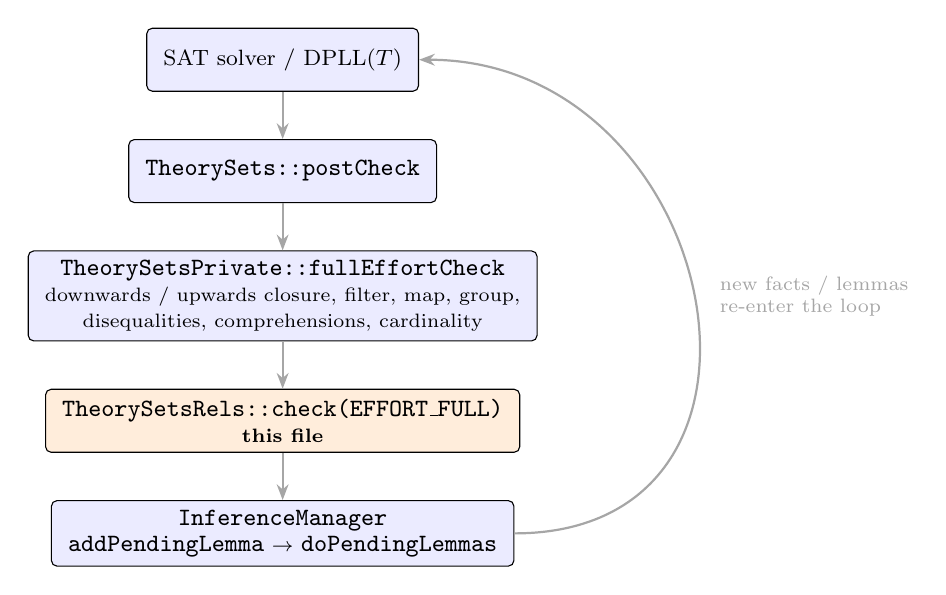
\begin{tikzpicture}[
  node distance=6mm,
  box/.style={draw,rounded corners=2pt,align=center,font=\footnotesize,
              minimum height=8mm,inner xsep=6pt},
  dark/.style={box,fill=blue!8},
  hot/.style={box,fill=orange!14},
  ar/.style={-{Stealth[length=2mm]},thick,gray!70}
]
\node[dark] (sat) {SAT solver / DPLL($T$)};
\node[dark,below=of sat] (th) {\code{TheorySets::postCheck}};
\node[dark,below=of th] (fe) {\code{TheorySetsPrivate::fullEffortCheck}\\
      \scriptsize downwards / upwards closure, filter, map, group,\\
      \scriptsize disequalities, comprehensions, cardinality};
\node[hot,below=of fe] (rels) {\code{TheorySetsRels::check(EFFORT\_FULL)}\\
      \scriptsize \textbf{this file}};
\node[dark,below=of rels] (im) {\code{InferenceManager}\\
      \scriptsize \code{addPendingLemma} $\to$ \code{doPendingLemmas}};
\draw[ar] (sat)--(th); \draw[ar] (th)--(fe); \draw[ar] (fe)--(rels);
\draw[ar] (rels)--(im);
\draw[ar] (im.east) to[out=0,in=0,looseness=1.6] node[right,font=\scriptsize,
      align=left,xshift=2mm]{new facts / lemmas\\ re-enter the loop} (sat.east);
\end{tikzpicture}
\caption{Position of the relational solver in the sets check loop.}
\end{figure}

\noindent
Two consequences of this placement matter throughout:

\begin{enumerate}[leftmargin=*,itemsep=2pt]
\item \textbf{The equality engine is the source of truth.} The relational
  solver never stores assertions of its own. At the beginning of every
  full-effort call it rebuilds all of its indices by walking the equality
  engine (\fn{collectRelsInfo}), and at the end it throws them away. All of the
  ``caches'' in the header are therefore \emph{scratch space for one call}, not
  persistent state.
\item \textbf{Nothing is asserted directly.} Conclusions are accumulated as
  pending lemmas via \fn{sendInfer} and flushed by
  \code{d\_im.doPendingLemmas()} after \fn{check} returns. A rule application
  is thus never immediately visible to a later rule in the same call; it
  becomes visible in the \emph{next} full-effort call, once the SAT solver has
  propagated it. This is why the file re-derives so much on every call, and why
  ``how many times do we compute this graph per call'' is a meaningful
  question.
\end{enumerate}

%%==========================================================================
\part{Data structures}\label{part:ds}
%%==========================================================================

\section{\code{TupleTrie}: an index of the members of a relation}

\begin{lstlisting}
class TupleTrie {
 public:
  std::map<Node, TupleTrie> d_data;
  std::vector<Node> findTerms(std::vector<Node>& reps, int argIndex = 0);
  std::vector<Node> findSuccessors(std::vector<Node>& reps, int argIndex = 0);
  Node existsTerm(std::vector<Node>& reps, int argIndex = 0);
  bool addTerm(Node n, std::vector<Node>& reps, int argIndex = 0);
};
\end{lstlisting}

\noindent
A \code{TupleTrie} is a prefix tree over the \emph{equivalence-class
representatives} of a tuple's components. For a tuple
$t = \tup{e_1,\dots,e_n}$ the path is
$\rep{e_1}\to\rep{e_2}\to\cdots\to\rep{e_n}\to t$: note the extra final level,
which stores the tuple term itself as a key with an empty subtrie. That is what
the comment ``\code{d\_data[n].clear()} \dots\ interpreted as the data and not
as a reference to a child'' in \fn{addTerm} means.

\begin{figure}[h]\centering
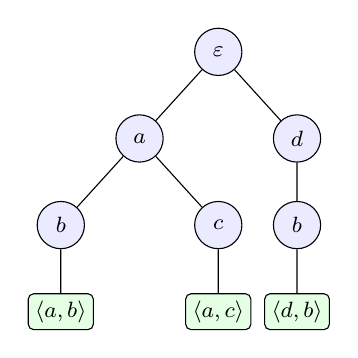
\begin{tikzpicture}[
  level distance=11mm, sibling distance=20mm,
  every node/.style={font=\footnotesize},
  n/.style={draw,circle,inner sep=1.4pt,minimum size=6mm,fill=blue!8},
  d/.style={draw,rectangle,rounded corners=2pt,inner sep=2.5pt,fill=green!10},
  e/.style={-{Stealth[length=1.6mm]},gray!70}
]
\node[n] (root) {$\varepsilon$}
  child {node[n] (a) {$a$}
    child {node[n] (ab) {$b$} child {node[d] {$\tup{a,b}$}}}
    child {node[n] (ac) {$c$} child {node[d] {$\tup{a,c}$}}}}
  child {node[n] (d) {$d$}
    child {node[n] (db) {$b$} child {node[d] {$\tup{d,b}$}}}};
\end{tikzpicture}
\caption{\code{d\_membership\_trie[$\rep{R}$]} after asserting
$\tup{a,b},\tup{a,c},\tup{d,b}\in R$. Round nodes are component
representatives; the boxed leaves are the stored tuple terms.}
\label{fig:trie}
\end{figure}

\noindent
The four operations differ only in where they stop and what they return:

\begin{center}\small
\begin{tabular}{@{}llp{7.6cm}@{}}
\toprule
Method & Stops at & Returns\\
\midrule
\fn{addTerm}\code{(n,reps)} & level $|reps|$ & inserts \code{n} as the leaf key;
  \code{false} if a tuple with the same representative vector is already
  present (this is the de-duplication used by \fn{collectRelsInfo}).\\
\fn{existsTerm}\code{(reps)} & level $|reps|$ & the stored tuple, or
  \code{null}: ``is there already a member with exactly these component
  representatives?''\\
\fn{findSuccessors}\code{(reps)} & level $|reps|$ & \emph{all keys one level
  below the given prefix}. With \code{reps} a 1-element prefix $[\rep{x}]$ over
  a binary relation, this is the set of $y$ with $\tup{x,y}\in R$ --- exactly
  what \code{RELATION\_JOIN\_IMAGE} needs.\\
\fn{findTerms}\code{(reps)} & level $|reps|-1$ & all keys at the last component
  level, \emph{but only if} \code{reps.back()} is a \code{SKOLEM} or
  \code{DUMMY\_SKOLEM}. In other words the last component acts as a wildcard
  when it is a Skolem. This is used by \fn{applyJoinRule} to enumerate the
  possible witnesses $z$ of \textsc{Join Down}.\\
\bottomrule
\end{tabular}
\end{center}

\begin{sidenote}
\fn{findTerms} returns the empty vector when the last component is \emph{not} a
Skolem. It is only ever called with a tuple whose last element is the freshly
created join witness, so this is intentional --- but it is a sharp edge if the
function is ever reused elsewhere.
\end{sidenote}

\section{The fields of \code{TheorySetsRels}}

Table~\ref{tab:fields} lists every member. The ``life'' column is the single
most useful thing to know about each: \emph{call} means the field is cleared at
the end of \fn{check()} (lines 215--224 of \file{theory\_sets\_rels.cpp});
\emph{object} means it is never cleared; \emph{user} means it is a
context-dependent container that backtracks with the user context.

\begin{center}\small
\renewcommand{\arraystretch}{1.22}
\begin{longtable}{@{}p{4.35cm}p{1.0cm}p{9.4cm}@{}}
\toprule
Field & Life & Meaning\\
\midrule\endhead
\code{d\_shared\_terms}\newline\scriptsize\code{CDHashSet<Node>} & user &
  Element terms for which a proxy singleton has already been requested from the
  term registry, so that theory combination will be told about them.
  Context-dependent because the proxy lemma is asserted in the user context.\\
\code{d\_rel\_nodes}\newline\scriptsize\code{unordered\_set<Node>} & call &
  Relational terms whose ``upward'' member computation has already run in this
  call. A pure idempotence guard: it makes
  \fn{computeMembersFor\dots} run at most once per term per call, no matter how
  many memberships trigger it.\\
\code{d\_tuple\_reps}\newline\scriptsize\code{map<Node,\allowbreak{}vector<Node>>} & call &
  Memoised component-representative vector of a tuple, i.e.\ the key used to
  address a \code{TupleTrie}. Filled by \fn{computeTupleReps}.\\
\code{d\_membership\_trie}\newline\scriptsize\code{map<Node,TupleTrie>} & call &
  Per relation \emph{representative}, the trie of Fig.~\ref{fig:trie} over its
  asserted members.\\
\code{d\_symbolic\_tuples}\newline\scriptsize\code{unordered\_set<Node>} &
  object &
  \code{SET\_MEMBER} nodes whose element argument was a bare variable and which
  have already been replaced by an explicit tuple constructor
  (\fn{reduceTupleVar}). Never cleared, and correctly so: the reduction lemma
  is a tautology, so emitting it once is enough for the whole solve.\\
\code{d\_rReps\_\allowbreak{}memberReps\_cache}\newline\scriptsize\code{map<Node,\allowbreak{}vector<Node>>}
  & call &
  \textbf{The membership index.} Maps a relation's representative $\rho$ to the
  list of \emph{tuple representatives} currently asserted to be in it.\\
\code{d\_rReps\_\allowbreak{}memberReps\_\allowbreak{}exp\_cache}\newline\scriptsize\code{map<Node,\allowbreak{}vector<Node>>}
  & call &
  The parallel array of \emph{explanations}: entry $i$ is the literal
  \code{(set.member $t$ $s$)} that justifies member $i$. Note $t$ and $s$ are
  the terms as they were asserted, \emph{not} representatives; the gap between
  $s$ and the relation being reasoned about is closed by adding an equality to
  every explanation.\\
\code{d\_terms\_cache}\newline\scriptsize\code{map<Node,\allowbreak{}map<Kind,\allowbreak{}vector<Node>>>}
  & call &
  For each set-of-tuples equivalence class, the relational-operator terms in
  it, bucketed by kind. This is how the solver finds ``the relational terms
  that are equal to the relation this membership is about''.\\
\code{d\_rRep\_tcGraph}\newline\scriptsize\code{map<Node,\allowbreak{}map<Node,\allowbreak{}set<Node>>>} &
  call &
  For a base relation representative $\rho$: the directed graph $G_\rho$ whose
  edges are exactly $\rho$'s asserted members. \emph{Read only by
  \fn{isTCReachable}.}\\
\code{d\_tcr\_tcGraph}\newline\scriptsize\code{map<Node,\allowbreak{}map<Node,\allowbreak{}set<Node>>>} &
  call &
  For a closure \emph{term} $T=\tc{r}$: the working graph $G_T$. Starts as a
  copy of $G_{\rep{r}}$ and is augmented with edges coming from asserted
  members of $T$ itself. \emph{Read only by \fn{doTCInference}.}\\
\code{d\_tcr\_tcGraph\_exps}\newline\scriptsize\code{map<Node,\allowbreak{}map<Node,Node>>} &
  call &
  For a closure term $T$: the explanation of each edge of $G_T$, keyed by the
  reconstructed pair term $\tup{a,b}$.\\
\bottomrule
\end{longtable}
\label{tab:fields}
\end{center}

\subsection{Two maps that are easy to confuse}

\code{d\_rRep\_tcGraph} is keyed by the \emph{base relation's representative};
\code{d\_tcr\_tcGraph} is keyed by the \emph{closure term itself}. They are
initialised to the same graph but they are not the same map and they diverge:

\begin{center}\small
\begin{tabular}{@{}lll@{}}
\toprule
 & \code{d\_rRep\_tcGraph[$\rep{r}$]} & \code{d\_tcr\_tcGraph[$\tc{r}$]}\\
\midrule
edges from members of $r$      & yes & yes\\
edges from members of $\tc{r}$ & \textbf{no} & \textbf{yes}\\
read by                        & \fn{isTCReachable} & \fn{doTCInference}\\
purpose & ``is this already derivable?'' & ``what can I derive?''\\
\bottomrule
\end{tabular}
\end{center}

\noindent
Keeping edges of $\tc{r}$ out of \code{d\_rRep\_tcGraph} is essential: that map
answers the question ``can I skip the expensive \textsc{TClos Down} splitting
lemma for this membership, because it already follows from $r$?''. If closure
edges leaked into it, the solver would suppress the splitting lemma for a
membership it had merely \emph{assumed}, which is circular.

\begin{sidenote}
Because \code{RelsUtils::constructPair(rel,a,b)} builds the pair from the
\emph{sort} of \code{rel} only, the pair terms produced with \code{rel\_rep},
\code{tc\_rel} and \code{tc\_rel[0]} are the very same node. That is why keys
written by \fn{buildTCGraphForRel} (which uses \code{rel\_rep}) can be looked up
by \fn{doTCInference} (which uses \code{tc\_rel}). It works, but it relies on an
implicit coincidence.
\end{sidenote}

%%==========================================================================
\part{The algorithms}\label{part:algo}
%%==========================================================================

\section{The top level: \fn{check}}

\begin{balgo}{\fn{TheorySetsRels::check(Theory::Effort e)} --- lines 57--73}
\begin{algorithmic}[1]
\If{$\neg$\Call{fullEffort}{$e$}} \State \Return \Comment{nothing at lower efforts}
\EndIf
\State \Call{collectRelsInfo}{} \Comment{rebuild all indices from the equality engine}
\State \Call{check}{} \Comment{apply the rules, accumulate pending lemmas}
\State \code{d\_im.doPendingLemmas()} \Comment{flush}
\end{algorithmic}
\end{balgo}

\noindent
The workhorse is the no-argument \fn{check()} (lines 75--246). It has a short
preamble that materialises the transitive-closure graphs, then three phases
whose boundaries are exactly the down/up split of the calculus.

\begin{balgo}{\fn{TheorySetsRels::check()} --- lines 75--246}\label{alg:check}
\begin{algorithmic}[1]
\Statex \textbf{Phase 0 --- materialise every closure graph}
\ForAll{$(\rho, K) \in$ \code{d\_terms\_cache}}
  \ForAll{$T \in K[\textsc{tclosure}]$}
    \State \Call{buildTCGraphForRel}{$T$}
      \Comment{\textcolor{hl}{the only call site, see Part~\ref{part:tc}}}
  \EndFor
\EndFor
\Statex
\Statex \textbf{Phase A --- downward rules, driven by memberships}
\ForAll{$(\rho, \mathit{members}) \in$ \code{d\_rReps\_memberReps\_cache}}
  \ForAll{$i \in [0,|\mathit{members}|)$}
    \State $m \gets \mathit{members}[i]$;\quad
           $e \gets$ \code{d\_rReps\_\allowbreak{}memberReps\_\allowbreak{}exp\_cache}$[\rho][i]$
    \State $K \gets$ \code{d\_terms\_cache}$[\rho]$
      \Comment{relational terms equal to this relation}
    \If{$K$ has \textsc{transpose} terms $\mathit{tp}$}
       \State \Call{applyTransposeRule}{$\mathit{tp}$}
         \Comment{\textsc{Transp Eq}: all transposes here are equal}
       \State \Call{applyTransposeRule}{$\mathit{tp}[0],\rho,e$}
         \Comment{\textsc{Transp Down}}
    \EndIf
    \ForAll{$t \in K[\textsc{join}]$}       \State \Call{applyJoinRule}{$t,\rho,e$} \EndFor
    \ForAll{$t \in K[\textsc{table\_join}]$}\State \Call{applyTableJoinRule}{$t,\rho,e$} \EndFor
    \ForAll{$t \in K[\textsc{product}]$}    \State \Call{applyProductRule}{$t,\rho,e$} \EndFor
    \ForAll{$t \in K[\textsc{tclosure}]$}   \State \Call{applyTCRule}{$m,t,\rho,e$} \EndFor
    \ForAll{$t \in K[\textsc{join\_image}]$}\State \Call{applyJoinImageRule}{$m,t,e$} \EndFor
    \ForAll{$t \in K[\textsc{iden}]$}       \State \Call{applyIdenRule}{$m,t,e$} \EndFor
  \EndFor
\EndFor
\Statex
\Statex \textbf{Phase B --- upward rules, driven by terms}
\ForAll{$(\rho, K) \in$ \code{d\_terms\_cache}}
  \ForAll{$(k, \mathit{terms}) \in K$}
    \ForAll{$t \in \mathit{terms}$}
      \If{$k \in \{$\textsc{join}, \textsc{product}, \textsc{table\_join}$\}$}
        \State \Call{computeMembersForBinOpRel}{$t$}
      \ElsIf{$k = $ \textsc{transpose}} \State \Call{computeMembersForUnaryOpRel}{$t$}
      \ElsIf{$k = $ \textsc{join\_image}} \State \Call{computeMembersForJoinImageTerm}{$t$}
      \ElsIf{$k = $ \textsc{iden}} \State \Call{computeMembersForIdenTerm}{$t$}
      \EndIf
    \EndFor
  \EndFor
\EndFor
\Statex
\Statex \textbf{Phase C --- transitive closure forward inference}
\State \Call{doTCInference}{} \Comment{walk every $G_T$ and emit \textsc{TClos Up I/II}}
\Statex
\Statex \textbf{Cleanup}
\State clear \code{d\_tuple\_reps}, \code{d\_rReps\_\allowbreak{}memberReps\_\allowbreak{}exp\_cache},
       \code{d\_terms\_cache}, \code{d\_membership\_trie},
       \code{d\_rel\_nodes}, \code{d\_rReps\_memberReps\_cache},
       \code{d\_rRep\_tcGraph}, \code{d\_tcr\_tcGraph\_exps},
       \code{d\_tcr\_tcGraph}
\end{algorithmic}
\end{balgo}

\begin{sidenote}
Phase B used to be guarded by
\code{if (d\_rReps\_memberReps\_cache.find(t\_it->first) == \dots end())},
i.e.\ it only ran for equivalence classes with \emph{no} memberships. That
guard was removed in commit \code{3bcc47a3c} (``Fix upwards closure for
relations'', PR~\#7515, Nov 2021) because upward closure must run even for
classes that do have members. The removal was right for join/product/transpose.
It also made \fn{buildTCGraphForRel} run a second time for closure terms, which
is the subject of Part~\ref{part:tc}; Phase~0 above is the resolution of that
question, and it is why Phase~B no longer has a \textsc{tclosure} branch at all.
\end{sidenote}

\section{\fn{collectRelsInfo}: rebuilding the world}

\begin{balgo}{\fn{collectRelsInfo} --- lines 231--314}\label{alg:collect}
\begin{algorithmic}[1]
\ForAll{equivalence classes $c$ of the equality engine}
  \ForAll{terms $n \in c$}
    \If{$\mathrm{type}(c)=\mathsf{Bool}$ and $\rep{c}$ is a constant}
       \Comment{$c$ is the \textsf{true} or \textsf{false} class}
      \If{$n = $ \code{(set.member $t$ $s$)} and $s$ is a relation}
        \State $\hat t \gets \rep{t}$;\quad $\hat s \gets \rep{s}$
        \If{$t$ is a variable} \State \Call{reduceTupleVar}{$n$}
          \Comment{lemma: $n \Leftrightarrow \tup{t.1,\dots,t.k}\in s$} \EndIf
        \If{$\rep{c} = \textsf{true}$}
           \Comment{\textbf{negative memberships are ignored}}
          \If{\Call{safelyAddToMap}{\code{d\_rReps\_memberReps\_cache},$\hat s,\hat t$}}
            \State append $n$ to \code{d\_rReps\_\allowbreak{}memberReps\_\allowbreak{}exp\_cache}$[\hat s]$
            \State \Call{computeTupleReps}{$\hat t$}
            \State \code{d\_membership\_trie}$[\hat s]$.\Call{addTerm}{$\hat t$,
                   \code{d\_tuple\_reps}$[\hat t]$}
          \EndIf
        \EndIf
      \EndIf
    \ElsIf{$\mathrm{type}(c)$ is a set of tuples}
      \If{$\mathrm{kind}(n)$ is a relational operator}
        \State append $n$ to \code{d\_terms\_cache}$[\rep{c}][\mathrm{kind}(n)]$
      \EndIf
    \ElsIf{$\mathrm{type}(c)$ is a tuple, $n$ neither constant nor variable}
      \ForAll{components $e$ of $n$ that are not constants}
        \State \Call{makeSharedTerm}{$e$}
      \EndFor
    \EndIf
  \EndFor
\EndFor
\end{algorithmic}
\end{balgo}

\noindent
Three details deserve emphasis.

\paragraph{Only positive memberships are indexed.}
\code{reason} is computed for both polarities but only the \code{is\_true\_eq}
branch populates the caches. Negative memberships
$\tup{a,b}\notin R$ are handled entirely by the equality engine: a rule that
derives $\tup{a,b}\in R$ will make the literal both true and false, which is
the \textsc{Eq Unsat} rule of the paper.

\paragraph{Everything is keyed by representatives.}
$\hat s = \rep{s}$ and $\hat t = \rep{t}$. This is how equality reasoning gets
``compiled away'': if $R_1 \approx R_2$, both contribute members to the same
bucket, and \code{d\_terms\_cache} puts the relational terms of both into the
same bucket too. The price is that the explanations must later re-introduce the
equalities that were quotiented out --- see Section~\ref{sec:exps}.

\paragraph{De-duplication is semantic, not syntactic.}
\fn{safelyAddToMap} (lines 1664--1691) compares the candidate member against
every member already recorded using \fn{areEqual}, not \code{==}. \fn{areEqual}
(lines 1624--1659) is itself recursive on tuples and, as a side effect,
\emph{marks non-equal components as shared terms}. So the act of indexing a
membership can enqueue proxy lemmas for theory combination. This is deliberate:
the join and table-join rules need to be notified when two element terms become
equal, and the only way to get that notification is to make them shared.

\section{Explanations: the discipline that makes the rest work}
\label{sec:exps}

\begin{lstlisting}
void TheorySetsRels::sendInfer(Node fact, InferenceId id, Node reason) {
  Node lemma = nodeManager()->mkNode(Kind::IMPLIES, reason, fact);
  d_im.addPendingLemma(lemma, id);
}
\end{lstlisting}

\noindent
Every rule builds a \emph{reason} that must be a conjunction of literals that
currently hold, and the lemma sent is $\mathit{reason}\Rightarrow
\mathit{fact}$. Because the indices are keyed by representatives while the
explanations record the literals as asserted, essentially every rule ends with
the same three-line idiom:

\begin{lstlisting}
Node reason = exp;                       // exp is (set.member t s), asserted
if (rel != exp[1]) {                     // s is not syntactically our rel...
  reason = nm->mkNode(AND, reason,       // ...so add the equality that says
                      nm->mkNode(EQUAL, rel, exp[1]));   // they are the same
}
sendInfer(conclusion, InferenceId::..., reason);
\end{lstlisting}

\begin{invariant}[Explanation soundness]\label{inv:exp}
For every call \fn{sendInfer}$(f,\mathit{id},r)$, $r$ is a conjunction of
literals each of which is entailed by the current assertions (memberships taken
from \code{d\_rReps\_\allowbreak{}memberReps\_\allowbreak{}exp\_cache}, equalities that hold in the
equality engine), and $r \models_{\TR} f$.
\end{invariant}

\noindent
There is a safety net for the case where the reason turns out \emph{not} to be
entailed --- \fn{processInference} (lines 1594--1608) wraps such an inference
into the splitting lemma $\neg r \vee f$ instead of asserting $f$ as a fact.

\begin{sidenote}
\fn{processInference} is dead code in the current file: nothing calls it, since
\fn{sendInfer} sends everything as a lemma anyway. Likewise
\fn{doPendingInfers} is declared in the header but never defined, and the
header comments still describe a \code{d\_pending} vector that no longer
exists. Reading the header alone will mislead you here.
\end{sidenote}

\section{The non-closure rules}\label{sec:otherrules}

Each operator is implemented by a pair of functions. The table below is the
map from the paper to the code; the \code{InferenceId} column is what you will
see in \code{--stats} output and in \code{-t sets-rels} traces.

\begin{center}\small
\renewcommand{\arraystretch}{1.15}
\begin{tabular}{@{}lllp{4.1cm}@{}}
\toprule
Paper rule & Direction & Function & \code{InferenceId}\\
\midrule
\textsc{Transp Down} & down & \fn{applyTransposeRule}(rel,rep,exp) & \code{SETS\_RELS\_TRANSPOSE\_REV}\\
\textsc{Transp Up}   & up   & \fn{computeMembersForUnaryOpRel}     & \code{SETS\_RELS\_TRANSPOSE\_REV}\\
---                  & ---  & \fn{applyTransposeRule}(vector)      & \code{SETS\_RELS\_TRANSPOSE\_EQ}\\
\textsc{Prod Down}   & down & \fn{applyProductRule}                & \code{SETS\_RELS\_PRODUCT\_SPLIT}\\
\textsc{Prod Up}     & up   & \fn{composeMembersForRels}           & \code{SETS\_RELS\_PRODUCE\_COMPOSE}\\
\textsc{Join Down}   & down & \fn{applyJoinRule}                   & \code{SETS\_RELS\_JOIN\_SPLIT\_1/2}\\
\textsc{Join Up}     & up   & \fn{composeMembersForRels}           & \code{SETS\_RELS\_JOIN\_COMPOSE}\\
--- (tables)         & down & \fn{applyTableJoinRule}              & \code{SETS\_RELS\_TABLE\_JOIN\_DOWN}\\
--- (tables)         & up   & \fn{applyTableJoinUp}                & \code{SETS\_RELS\_TABLE\_JOIN\_UP}\\
--- (iden)           & down & \fn{applyIdenRule}                   & \code{SETS\_RELS\_IDENTITY\_DOWN}\\
--- (iden)           & up   & \fn{computeMembersForIdenTerm}       & \code{SETS\_RELS\_IDENTITY\_UP}\\
--- (join image)     & down & \fn{applyJoinImageRule}              & \code{SETS\_RELS\_JOIN\_IMAGE\_DOWN}\\
--- (join image)     & up   & \fn{computeMembersForJoinImageTerm}  & \code{SETS\_RELS\_JOIN\_IMAGE\_UP}\\
\textsc{TClos Down}  & down & \fn{applyTCRule}                     & \code{SETS\_RELS\_TCLOSURE\_UP}\\
\textsc{TClos Up I/II} & up & \fn{doTCInference}                   & \code{SETS\_RELS\_TCLOSURE\_FWD}\\
--- (tuple vars)     & ---  & \fn{reduceTupleVar}                  & \code{SETS\_RELS\_TUPLE\_REDUCTION}\\
\bottomrule
\end{tabular}
\end{center}

\begin{sidenote}
The \code{InferenceId} for \textsc{TClos Down} is called
\code{SETS\_RELS\_TCLOSURE\_UP} and the one for \textsc{TClos Up I/II} is called
\code{\dots\_FWD}. The naming is inverted with respect to the paper. Do not use
the identifiers to orient yourself.
\end{sidenote}

\subsection{Transpose}

\textsc{Transp Down} is a one-liner: reverse the tuple in \code{exp[0]} and
assert it in \code{tp\_rel[0]}. \textsc{Transp Up} iterates the members of
\code{rel[0]} and asserts the reverse of each in \code{rel}.

The extra rule, \fn{applyTransposeRule}\code{(vector<Node> tp\_terms)}, has no
counterpart in the paper. If two transpose terms $\transp{X}$ and $\transp{Y}$
are in the same equivalence class then $\transp{X}\approx\transp{Y}$, and since
transpose is injective, $X\approx Y$:
\[
\inferrule*[left=\textsc{Transp Eq}]
  {\transp{X}\approx\transp{Y}}{X\approx Y}
\]
Note that this is emitted once \emph{per member} of the equivalence class
(Algorithm~\ref{alg:check} calls it inside the member loop), so with $k$
members and $j$ transposes it enqueues $k(j-1)$ identical lemmas. They are
de-duplicated downstream, but the work is real.

\subsection{Product and join, downward}

Both split the member tuple. For product, the split is positional:
$\tup{x_1..x_m,y_1..y_n} \in R_1\prodop R_2$ yields
$\tup{x_1..x_m}\in R_1$ and $\tup{y_1..y_n}\in R_2$.
For join, a fresh Skolem $z$ is glued into the middle:

\begin{balgo}{\fn{applyJoinRule}$(J = R_1\join R_2,\ \rho,\ \mathit{exp})$ --- lines 1053--1132}
\begin{algorithmic}[1]
\If{$J \notin$ \code{d\_rel\_nodes}}
  \State \Call{computeMembersForBinOpRel}{$J$};\quad insert $J$ into \code{d\_rel\_nodes}
\EndIf
\State $\tup{a_1..a_{m-1},b_1..b_n} \gets \mathit{exp}[0]$
\State $z \gets$ \Call{mkTypedSkolemCached}{$\mathit{exp}[0], J$, \code{SK\_JOIN}}
  \Comment{same $(mem, J)$ $\Rightarrow$ same Skolem}
\State $t_1 \gets \tup{a_1..a_{m-1},z}$; \quad $t_2 \gets \tup{z,b_1..b_n}$
\Statex \Comment{\emph{redundancy check}: is a witness already present?}
\ForAll{$u \in$ \code{d\_membership\_trie}$[\rep{R_1}]$.\Call{findTerms}{$\mathrm{reps}(t_1)$}}
  \If{\code{d\_membership\_trie}$[\rep{R_2}]$.\Call{existsTerm}{$u\cdot\mathrm{reps}(t_2)_{2..}$} $\neq$ \code{null}}
     \State \Return \Comment{\textsc{Join Down} would be a redundant application}
  \EndIf
\EndFor
\State \Call{sendInfer}{$t_1 \in R_1$, \code{JOIN\_SPLIT\_1}, reason}
\State \Call{sendInfer}{$t_2 \in R_2$, \code{JOIN\_SPLIT\_2}, reason}
\State \Call{makeSharedTerm}{$z$}
\end{algorithmic}
\end{balgo}

\noindent
The \code{findTerms}/\code{existsTerm} pair implements the paper's
\emph{redundancy criterion} (``an application is redundant if $S$ already
contains $\varphi_1[x_1,t],\dots$ for some terms $t$''): if some $u$ already
witnesses the join for this member, do not introduce a new Skolem. Together
with the caching in \code{SkolemCache} --- the witness is keyed by the pair
(member, join term), so re-deriving the same membership reuses the same $z$ ---
this is what stops \textsc{Join Down} from generating an unbounded supply of
witnesses.

\subsection{Product and join, upward: \fn{composeMembersForRels}}

\fn{computeMembersForBinOpRel} first recurses into the arguments (so that a
nested $\transp{(X\join Y)}$ has its members computed bottom-up) and then calls
\fn{composeMembersForRels}, which is the quadratic double loop over the members
of $R_1$ and $R_2$. For join it must decide whether the ``middle'' elements
match:

\begin{center}
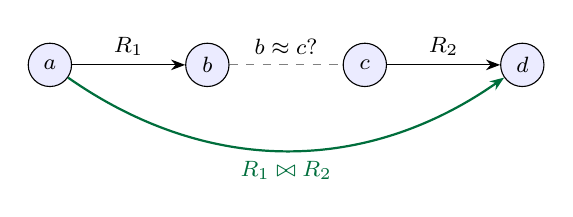
\begin{tikzpicture}[font=\footnotesize,
  n/.style={draw,circle,inner sep=1pt,minimum size=5.5mm,fill=blue!8},
  e/.style={-{Stealth[length=1.8mm]}}]
  \node[n] (a) at (0,0) {$a$};
  \node[n] (b) at (2,0) {$b$};
  \node[n] (c) at (4,0) {$c$};
  \node[n] (d) at (6,0) {$d$};
  \draw[e] (a)--node[above]{$R_1$}(b);
  \draw[e] (c)--node[above]{$R_2$}(d);
  \draw[dashed,gray] (b)--node[above,black]{$b \approx c$?}(c);
  \draw[e,bend right=35,thick,good] (a) to node[below]{$R_1\join R_2$} (d);
\end{tikzpicture}
\end{center}

\begin{itemize}[leftmargin=*,itemsep=1pt]
\item If $b$ and $c$ are currently equal: emit
  $\tup{a,d}\in R_1\join R_2$, adding $b\approx c$ to the reason when the two
  terms are syntactically different.
\item Otherwise: \emph{do nothing}, but call \fn{makeSharedTerm} on both $b$
  and $c$ first. Marking them shared hands the case split to theory
  combination, which will only split when it actually matters. This replaced an
  older implementation that emitted an explicit $b\approx c \vee b\not\approx c$
  lemma (see PR~\#7515); the comment in the code spells this out.
\end{itemize}

\subsection{Table join}

\code{RELATION\_TABLE\_JOIN} carries a \code{ProjectOp} with an index list
$m_1,n_1,\dots,m_k,n_k$ meaning ``column $m_i$ of the left tuple must equal
column $n_i$ of the right tuple''. \fn{applyTableJoinRule} is the downward rule:
from $e \in (A \bowtie_{\vec m,\vec n} B)$ it splits $e$ positionally into $a$
and $b$ and concludes $a\in A \wedge b\in B \wedge \bigwedge_i a_{m_i} \approx
b_{n_i}$. Unlike \textsc{Join Down} there is no Skolem, because the join columns
are explicit. \fn{applyTableJoinUp} is the matching quadratic upward rule.

\subsection{Identity}

$\mathsf{iden}(R) = \{\tup{x,x}\mid \tup{x}\in R\}$ with $R$ unary.
Downward (\fn{applyIdenRule}): from $\tup{x,y}\in\mathsf{iden}(R)$ conclude
$\tup{x}\in R \wedge x\approx y$. Upward
(\fn{computeMembersForIdenTerm}): from $\tup{x}\in R$ conclude
$\tup{x,x}\in\mathsf{iden}(R)$.

\subsection{Join image}

$R \mathbin{\mathsf{jimg}} n$ is the set of $\tup{x}$ having at least $n$
\emph{distinct} $R$-successors.

\begin{itemize}[leftmargin=*,itemsep=1pt]
\item \textbf{Down} (\fn{applyJoinImageRule}): from $\tup{x}\in
  R\mathbin{\mathsf{jimg}} n$ create $n$ fresh Skolems $k_1..k_n$ and conclude
  $\bigwedge_i \tup{x,k_i}\in R \wedge \mathrm{distinct}(k_1..k_n)$. It first
  short-circuits if the trie already shows $\ge n$ successors of $x$
  (\fn{findSuccessors}).
\item \textbf{Up} (\fn{computeMembersForJoinImageTerm}): scan the members of
  $R$, group them by first component, and as soon as $n$ pairwise-distinct
  second components have been seen for some $x$, conclude
  $\tup{x}\in R\mathbin{\mathsf{jimg}} n \vee \neg\mathrm{distinct}(y_1..y_n)$.
  The disjunction is needed because the $y_i$ were only checked to be
  \emph{not currently known equal}, not to be distinct.
\end{itemize}

%%==========================================================================
\section{Transitive closure in detail}\label{sec:tcdetail}
%%==========================================================================

Transitive closure is the only operator whose implementation is not a direct
transcription of two rules. It maintains an explicit graph, and the graph is
where the interesting invariants live.

\subsection{The idea}

Read a binary relation $r$ as a directed graph: an asserted membership
$\tup{a,b}\in r$ is an edge $a\to b$. Then
\[
  \tup{a,b} \in \tc{r} \iff \text{there is a path of length} \ge 1
  \text{ from } a \text{ to } b .
\]
\textsc{TClos Up I} says every edge is a path; \textsc{TClos Up II} says paths
compose. Instead of applying those two rules one step at a time --- which would
need one full-effort round per path edge --- the implementation materialises the
graph once and enumerates \emph{all} paths by depth-first search, emitting one
\code{SETS\_RELS\_TCLOSURE\_FWD} lemma per path. That is
\fn{doTCInference}.

Crucially, the graph is not built from the members of $r$ alone. Memberships in
$\tc{r}$ itself are also edges --- an assumed $\tup{a,b}\in \tc{r}$ can be
chained with anything else in $\tc{r}$ by \textsc{TClos Up II}. Those edges are
added by \fn{applyTCRule}.

\begin{figure}[h]\centering
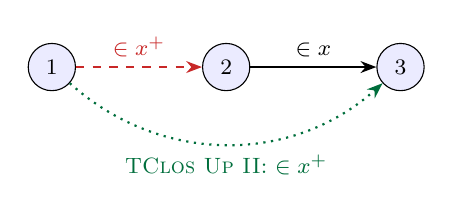
\begin{tikzpicture}[font=\footnotesize,node distance=16mm,
  n/.style={draw,circle,inner sep=1pt,minimum size=6mm,fill=blue!8},
  base/.style={-{Stealth[length=2mm]},thick},
  clos/.style={-{Stealth[length=2mm]},thick,dashed,hl},
  derived/.style={-{Stealth[length=2mm]},good,thick,dotted}]
  \node[n] (1) {$1$};
  \node[n,right=of 1] (2) {$2$};
  \node[n,right=of 2] (3) {$3$};
  \draw[clos] (1) -- node[above]{$\in\tc{x}$} (2);
  \draw[base] (2) -- node[above]{$\in x$} (3);
  \draw[derived] (1) to[bend right=42] node[below]{\textsc{TClos Up II}: $\in\tc{x}$} (3);
\end{tikzpicture}
\caption{$G_{\tc{x}}$ for the assertions
$\tup{2,3}\in x$, $\tup{1,2}\in\tc{x}$. Solid = edge of the base relation
(contributed by \fn{buildTCGraphForRel}), dashed = edge from an asserted
closure membership (contributed by \fn{applyTCRule}), dotted = what
\fn{doTCInference} derives from the path.}
\label{fig:tcmix}
\end{figure}

\subsection{\fn{buildTCGraphForRel}: materialising the base graph}

\begin{balgo}{\fn{buildTCGraphForRel}$(T)$ where $T=\tc{r}$ --- lines 830--877}\label{alg:build}
\begin{algorithmic}[1]
\State $\rho \gets \rep{r}$
\If{$\rho \notin$ \code{d\_rReps\_memberReps\_cache}}
  \State \Return \Comment{$r$ has no asserted member; nothing to build}
\EndIf
\State $\mathit{members} \gets$ \code{d\_rReps\_memberReps\_cache}$[\rho]$;\quad
       $\mathit{exps} \gets$ \code{d\_rReps\_\allowbreak{}memberReps\_\allowbreak{}exp\_cache}$[\rho]$
\State $G \gets \emptyset$; \quad $E \gets \emptyset$
\ForAll{$i \in [0,|\mathit{members}|)$}
  \State $u \gets \rep{\mathit{members}[i].1}$; \quad $v \gets \rep{\mathit{members}[i].2}$
  \If{$v \notin G[u]$}
    \State $G[u] \gets G[u] \cup \{v\}$;\quad $E[\tup{u,v}] \gets \mathit{exps}[i]$
  \EndIf
\EndFor
\If{$|\mathit{members}| > 0$}
  \State \code{d\_rRep\_tcGraph}$[\rho] \gets G$
    \Comment{base graph, for \fn{isTCReachable}}
  \State \code{d\_tcr\_tcGraph}$[T] \;\;\;\gets G$
    \Comment{\textcolor{hl}{\textbf{overwrites}} whatever was there}
  \State \code{d\_tcr\_tcGraph\_exps}$[T] \gets E$
    \Comment{\textcolor{hl}{\textbf{overwrites}}}
\EndIf
\end{algorithmic}
\end{balgo}

\noindent
Two things to notice. First, the function is a pure function of
\code{d\_rReps\_memberReps\_cache}, which \fn{collectRelsInfo} fills and no rule
subsequently modifies. \emph{Calling it at any point during \fn{check()}
therefore produces exactly the same graph.} Second, the three assignments at the
end are plain \code{operator[]} assignments: they replace, they do not merge.
Remember this for Part~\ref{part:tc} --- it is the whole story of that part.

\begin{sidenote}
The early return on line 2 is new. Until \code{8bcdf3239} the function read
\code{d\_rReps\_memberReps\_cache[rel\_rep]} and
\code{d\_rReps\_memberReps\_exp\_cache[rel\_rep]} with \code{operator[]}, which
\emph{inserts} an empty vector when $r$ has no asserted member. Two maps that
Phase~A iterates were therefore silently mutated by a graph build, and every
later \code{find($\rho$) != end()} test on them --- the standard ``does this
relation have members?'' idiom in this file, used by
\fn{computeMembersForJoinImageTerm}, \fn{computeMembersForIdenTerm},
\fn{applyTransposeRule} and \fn{composeMembersForRels} --- reported a false
positive for $\rho$. Those callers happen to survive it, because they go on to
iterate a vector that is empty, but the idiom was lying. The same commit dropped
the unused local \code{tc\_rel\_rep}.
\end{sidenote}

\subsection{\fn{applyTCRule}: \textsc{TClos Down} plus graph augmentation}
\label{sec:tcrule}

\begin{balgo}{\fn{applyTCRule}$(m, T, \rho, \mathit{exp})$ where $T=\tc{r}$ --- lines 648--758}\label{alg:tcrule}
\begin{algorithmic}[1]
\Statex \Comment{$G_T$ was built in Phase~0; this rule only ever adds to it}
\If{\Call{isTCReachable}{$m, T$}}
  \State \Return \Comment{already entailed; do not split}
\EndIf
\State $a \gets \rep{m.1}$; \quad $b \gets \rep{m.2}$
\State add edge $a\to b$ to \code{d\_tcr\_tcGraph}$[T]$ and
       $\mathit{exp}$ to \code{d\_tcr\_tcGraph\_exps}$[T][\tup{a,b}]$
\Statex \Comment{now the branching rule, with cached Skolems $s_1,s_2$}
\State $\tup{x,y} \gets \mathit{exp}[0]$
\State $s_1 \gets$ \code{SK\_TCLOSURE\_DOWN1}$(\mathit{exp}[0], r)$;\quad
       $s_2 \gets$ \code{SK\_TCLOSURE\_DOWN2}$(\mathit{exp}[0], r)$
\State \Call{sendInfer}{$\;\tup{x,y}\in r \;\vee\;
   \big(\tup{x,s_1}\in r \wedge \tup{s_2,y}\in r \wedge
        (s_1\approx s_2 \vee \tup{s_1,s_2}\in T)\big)$,
   \code{TCLOSURE\_UP}, reason}
\end{algorithmic}
\end{balgo}

\noindent
The conclusion is the paper's \textsc{TClos Down} with the three branches
refactored into two: branch~2 ($\tup{x,z}\in r,\tup{z,y}\in r$) and branch~3
($\tup{x,z_1}\in r, \tup{z_1,z_2}\in\tc{r},\tup{z_2,y}\in r, z_1\not\approx
z_2$) share the shape $\tup{x,s_1}\in r \wedge \tup{s_2,y}\in r$ and are
distinguished by $s_1 \approx s_2$ (branch 2, the two-step case) versus
$\tup{s_1,s_2}\in\tc{r}$ (branch 3). Note the code does \emph{not} assert
$s_1\not\approx s_2$ in branch 3, so the two branches overlap; that is harmless
for soundness and avoids a disequality.

Termination pressure comes from three places, and it is worth being explicit
about them because they are the only thing standing between this rule and an
infinite regress:

\begin{enumerate}[leftmargin=*,itemsep=1pt]
\item \textbf{Skolem caching.} $s_1,s_2$ are produced by
  \code{SkolemCache::mkTypedSkolemCached} keyed on $(\mathit{exp}[0], r)$ and a
  purpose tag, so re-processing the same membership in a later round reuses the
  same two Skolems. Without this, every round would invent new nodes.
\item \textbf{The reachability guard.} If $m$ is already a member of $r$, or is
  connected in $G_{\rep r}$, the rule returns before splitting.
\item \textbf{Graph augmentation.} Recording $a\to b$ means the same
  membership can be discharged by \fn{doTCInference} instead of by splitting on
  a later round.
\end{enumerate}

\begin{sidenote}
Until \code{8bcdf3239} this rule opened with a build of its own, under the guard
\code{d\_rReps\_memberReps\_cache.find(tc\_rel[0]) != end() \&\& tc\_rel
$\notin$ d\_rel\_nodes \&\& getRepresentative(tc\_rel[0]) $\notin$
d\_rRep\_tcGraph}. Note the first clause looked up \code{tc\_rel[0]}, the term
itself, where \fn{buildTCGraphForRel} looks up its
\emph{representative}: when $r$ was not its own representative the guard was
simply false, no graph was built here, and \fn{isTCReachable} below ran against
nothing --- so the rule emitted a splitting lemma for a membership the graph
would have discharged. Phase~0 sidesteps the whole question by building
unconditionally, before any rule can look.
\end{sidenote}

\subsection{\fn{isTCReachable}: the entailment guard}

\begin{balgo}{\fn{isTCReachable}$(m, T)$ --- lines 747--776}
\begin{algorithmic}[1]
\If{$m$ occurs in \code{d\_rReps\_memberReps\_cache}$[\rep{r}]$}
  \State \Return \textbf{true} \Comment{$m\in r$, so $m\in\tc{r}$ by \textsc{TClos Up I}}
\EndIf
\If{$\rep{r} \in$ \code{d\_rRep\_tcGraph}}
  \State \Return DFS from $\rep{m.1}$ to $\rep{m.2}$ in
         \code{d\_rRep\_tcGraph}$[\rep{r}]$
\EndIf
\State \Return \textbf{false}
\end{algorithmic}
\end{balgo}

\noindent
The DFS is the second \fn{isTCReachable} overload (lines 778--814): standard
depth-first search with a \code{hasSeen} set, writing its answer into a
by-reference \code{bool}. Two small inefficiencies: the loop does not break once
\code{isReachable} becomes true in a recursive call, and the caller applies
\code{getRepresentative} twice to the same node.

Note the graph consulted is \code{d\_rRep\_tcGraph}, the \emph{base} graph. This
is the asymmetry described in Part~\ref{part:ds}: it must not see edges that
came from assumed $\tc{r}$ memberships, otherwise a membership would justify
suppressing its own splitting lemma.

\subsection{\fn{doTCInference}: enumerating paths}

Phase~C consists of three overloads that form a driver / per-graph / recursive
triple.

\begin{balgo}{\fn{doTCInference} (three overloads) --- lines 1255--1273, 860--897, 899--978}
\begin{algorithmic}[1]
\Function{doTCInference}{} \Comment{driver, line 1255}
  \ForAll{$(T, G) \in$ \code{d\_tcr\_tcGraph}}
    \State \Call{doTCInference}{$G$, \code{d\_tcr\_tcGraph\_exps}$[T]$, $T$}
  \EndFor
\EndFunction
\Statex
\Function{doTCInference}{$G$, $E$, $T$} \Comment{per graph, line 860}
  \ForAll{$u \in \mathrm{dom}(G)$}
    \ForAll{$v \in G[u]$}
      \State \Call{dfs}{$T$, $[\,E[\tup{u,v}]\,]$, $G$, $E$, $u$, $v$, $\{u\}$}
    \EndFor
  \EndFor
\EndFunction
\Statex
\Function{dfs}{$T$, \emph{reasons}, $G$, $E$, \emph{start}, \emph{cur}, \emph{seen}}
  \Comment{line 899}
  \State $x \gets \mathit{reasons}.\mathrm{front}()[0].1$;\quad
         $y \gets \mathit{reasons}.\mathrm{back}()[0].2$
  \State \emph{all} $\gets$ \emph{reasons}
  \ForAll{consecutive pairs $(\ell_i,\ell_{i+1})$ in \emph{reasons}}
    \If{$\ell_i[0].2 \neq \ell_{i+1}[0].1$}
      \State append $\ell_i[0].2 \approx \ell_{i+1}[0].1$ to \emph{all}
        \Comment{stitch the chain}
    \EndIf
    \If{$T \neq \ell_i[1]$ \textbf{and} $r \neq \ell_i[1]$}
      \State append $r \approx \ell_i[1]$ to \emph{all}
        \Comment{the literal was about an equal relation}
    \EndIf
  \EndFor
  \State (same relation-equality fix-up for $\mathit{reasons}.\mathrm{back}()$)
  \State \Call{sendInfer}{$\tup{x,y}\in T$, \code{TCLOSURE\_FWD},
         $\bigwedge \mathit{all}$}
  \Statex
  \If{$\mathit{cur} \in \mathit{seen}$} \State \Return \EndIf
  \State $\mathit{seen} \gets \mathit{seen}\cup\{\mathit{cur}\}$
  \ForAll{$w \in G[\mathit{cur}]$}
    \State \Call{dfs}{$T$, $\mathit{reasons}\cdot E[\tup{\mathit{cur},w}]$,
           $G$, $E$, \emph{start}, $w$, \emph{seen}}
  \EndFor
\EndFunction
\end{algorithmic}
\end{balgo}

\noindent
\emph{reasons} is the chain of membership literals along the current path; the
conclusion is always ``first element of the first literal'' to ``second element
of the last literal''. Two subtleties:

\begin{itemize}[leftmargin=*,itemsep=1pt]
\item The endpoints $x,y$ are read from the \emph{literals}, not from the graph
  nodes. Graph nodes are representatives, but the literals mention the original
  terms; taking the endpoints from the literals is what makes the emitted
  membership talk about terms the rest of the solver has seen. The equalities
  appended in the loop close the gap between consecutive links.
\item \code{seen} is passed \emph{by reference} and is shared across siblings in
  the DFS. It therefore behaves as a global visited-set for the whole traversal
  rooted at one edge, not as a path-local set. This makes the traversal linear
  rather than exponential, at the cost of not enumerating every simple path ---
  a deliberate under-approximation. Since every emitted lemma is sound, missing
  some paths only costs completeness of the round, and the missing memberships
  are typically re-derived on later rounds from the newly asserted ones.
\end{itemize}

\begin{example}[The graph of Figure~\ref{fig:tcmix}]
$G_{\tc{x}} = \{1\mapsto\{2\},\ 2\mapsto\{3\}\}$ with
$E[\tup{1,2}] = (\tup{1,2}\in\tc{x})$, $E[\tup{2,3}]=(\tup{2,3}\in x)$.
The driver visits $u=1$: \code{dfs} with reasons $[\tup{1,2}\in\tc{x}]$ emits
$\tup{1,2}\in\tc{x}$ (trivial), then recurses to $\mathit{cur}=2$ with reasons
$[\tup{1,2}\in\tc{x},\ \tup{2,3}\in x]$ and emits
\[
  \tup{1,2}\in\tc{x} \wedge \tup{2,3}\in x \;\Rightarrow\; \tup{1,3}\in\tc{x},
\]
which together with an assertion $\tup{1,3}\notin\tc{x}$ closes the branch.
\end{example}

\subsection{The transitive-closure invariants}

\begin{invariant}[Node domain]\label{inv:nodes}
Every vertex of \code{d\_rRep\_tcGraph}$[\rho]$ and of
\code{d\_tcr\_tcGraph}$[T]$ is an equivalence-class representative of an element
term. Consequently two currently-equal elements are the \emph{same} vertex, and
graph reachability already accounts for equality reasoning.
\end{invariant}

\begin{invariant}[Base graph]\label{inv:base}
\code{d\_rRep\_tcGraph}$[\rho] = \{\,\rep{a}\to\rep{b} \mid \tup{a,b}$ is an
asserted member of the class $\rho\,\}$ --- edges of the \emph{base relation
only}, never of a closure term.
\end{invariant}

\begin{invariant}[Working graph soundness]\label{inv:sound}
For $T = \tc{r}$, every edge $a\to b$ of \code{d\_tcr\_tcGraph}$[T]$ satisfies
$\tup{a,b}\in T$ under the current assertions: either $\tup{a,b}$ is an asserted
member of $r$'s class (\textsc{TClos Up I}) or an asserted member of $T$'s
class. Hence \emph{every path in $G_T$ from $a$ to $b$ witnesses
$\tup{a,b}\in T$} by \textsc{TClos Up II}, and the chain of edge explanations is
a valid reason for it.
\end{invariant}

\begin{invariant}[Working graph completeness]\label{inv:complete}
$\;$\code{d\_tcr\_tcGraph}$[T] \supseteq$ \code{d\_rRep\_tcGraph}$[\rep{r}]$,
\emph{and} contains an edge for every asserted member of $T$ that
\fn{isTCReachable} did not already discharge.
\end{invariant}

\begin{invariant}[Explanation totality]\label{inv:tot}
$\mathrm{dom}($\code{d\_tcr\_tcGraph\_exps}$[T])\;\supseteq\;$ the edge set of
\code{d\_tcr\_tcGraph}$[T]$, with keys built by
\code{RelsUtils::constructPair}. \fn{doTCInference} dereferences
\code{find(new\_pair)->second} without a null check, so a violation of this
invariant is undefined behaviour, not a wrong answer.
\end{invariant}

\begin{invariant}[Lifetime]\label{inv:life}
All three TC maps are scratch for a single \fn{check()} call and are cleared at
lines 243--245. Nothing in them survives to the next full-effort round.
\end{invariant}

\noindent
Invariants~\ref{inv:nodes}, \ref{inv:base}, \ref{inv:sound}, \ref{inv:tot} and
\ref{inv:life} hold in any arrangement of the code. Invariant~\ref{inv:complete}
is the delicate one: it holds with Phase~0 by construction, because the only
assignment to \code{d\_tcr\_tcGraph}$[T]$ happens before any rule runs and
everything afterwards is an insertion, whereas on \code{main} it takes a
guard at each of two call sites and holds only per base relation. That is the
subject of the next part.

%%==========================================================================
\part{Should \fn{buildTCGraphForRel} be called once or twice?}\label{part:tc}
%%==========================================================================

\section{The question}

On \code{main} (\code{5cc03f4b9}, whose line numbers this section quotes),
\fn{buildTCGraphForRel} has two call sites, each guarded:

\begin{center}\small
\begin{tabular}{@{}llp{7.4cm}@{}}
\toprule
& Site & Guard\\
\midrule
$\bigstar_1$ & \fn{applyTCRule}, line 645 &
  \code{d\_rReps\_memberReps\_cache} contains \code{tc\_rel[0]}
  \textbf{and} \code{tc\_rel} $\notin$ \code{d\_rel\_nodes}
  \textbf{and} $\rep{\code{tc\_rel[0]}} \notin$ \code{d\_rRep\_tcGraph}\\
$\bigstar_2$ & \fn{check()} Phase~B, line 191 &
  \code{*term\_it} $\notin$ \code{d\_rel\_nodes}
  \textbf{and} $\rep{\code{(*term\_it)[0]}} \notin$ \code{d\_rRep\_tcGraph}\\
\bottomrule
\end{tabular}
\end{center}

\noindent
in code:

\begin{lstlisting}
// Protect d_tcr_tcGraph from being overwritten, if it already exists
if (d_rel_nodes.find(*term_it) == d_rel_nodes.end()
    && d_rRep_tcGraph.find(getRepresentative((*term_it)[0]))
           == d_rRep_tcGraph.end())
{
  buildTCGraphForRel(*term_it);
  d_rel_nodes.insert(*term_it);
}
\end{lstlisting}

\noindent
The two maps in those conditions are not being consulted for their contents;
they are being used as ``a graph for this relation has already been built''
markers, and the comment says what they are protecting against. So the guards
are not an optimisation, they are the mechanism that keeps the second call from
destroying the first call's work (Observation~\ref{obs:destroy} below). The
question of this part is whether to keep that arrangement or to replace both
sites with a single unconditional pass immediately after \fn{collectRelsInfo}.

\code{main} is correct on everything measured here
(Section~\ref{sec:measure}), so what follows is not a bug report. Two properties
distinguish the two configurations:

\begin{itemize}[leftmargin=*,itemsep=2pt]
\item \textbf{Which call builds is decided by iteration order.} The outcome
  depends on whether Phase~A reached $T$ before Phase~B did. Correctness is
  preserved by the facts that Phase~A always runs first and that $\bigstar_1$
  builds before it augments --- a two-site argument, where one call needs no
  argument at all.
\item \textbf{The guards are keyed by base representative, not by term.} If two
  closure terms $\tc{x}$ and $\tc{y}$ have $x \approx y$, the second of them
  never receives the base edges in \code{d\_tcr\_tcGraph}, only whatever
  $\bigstar_1$ later inserts. Invariant~\ref{inv:complete} fails for that term.
  This is benign --- the two closure terms are congruent, so the memberships
  derived for the first propagate --- and it is unobservable in the test suite,
  but it is a weaker statement than the invariant.
\end{itemize}

\section{Static analysis}

\begin{observation}[The graph does not depend on when it is built]
\code{d\_rReps\_memberReps\_cache} and
\code{d\_rReps\_\allowbreak{}memberReps\_\allowbreak{}exp\_cache} are written only by
\fn{collectRelsInfo}. No rule in Phase~A or Phase~B adds a member to them
(rules only enqueue \emph{lemmas}, which become visible in the next
full-effort round). \fn{buildTCGraphForRel} reads nothing else. Therefore
$\bigstar_1$ and $\bigstar_2$ compute \textbf{bit-identical} graphs, and a
single call placed anywhere before Phase~C computes the same graph too.
\end{observation}

\begin{observation}[A second call would be destructive]\label{obs:destroy}
Between $\bigstar_1$ and $\bigstar_2$, \fn{applyTCRule} adds edges to
\code{d\_tcr\_tcGraph}$[T]$ for the asserted members of $T$ itself
(Algorithm~\ref{alg:tcrule}, line 8). Were $\bigstar_2$ to run, it would execute
\code{d\_tcr\_tcGraph[tc\_rel] = rel\_tc\_graph}, a whole-map assignment, and
\textbf{all of those edges would be discarded}, together with their
explanations. This is what the guards on \code{main} exist to prevent, and it is
why they cannot be dropped while the call site remains.
\end{observation}

\noindent
So the second call is not a redundant recomputation of the same thing. It is a
recomputation of a \emph{smaller} thing that would overwrite a larger one. The
only reason the resulting bug was survivable for as long as it was is
\code{if (members.size() > 0)} inside \fn{buildTCGraphForRel}: the damage needs
the base relation to have at least one asserted member, and most
transitive-closure regressions assert memberships in $\tc{r}$ or in $r$ but
rarely both.

\begin{figure}[h]\centering
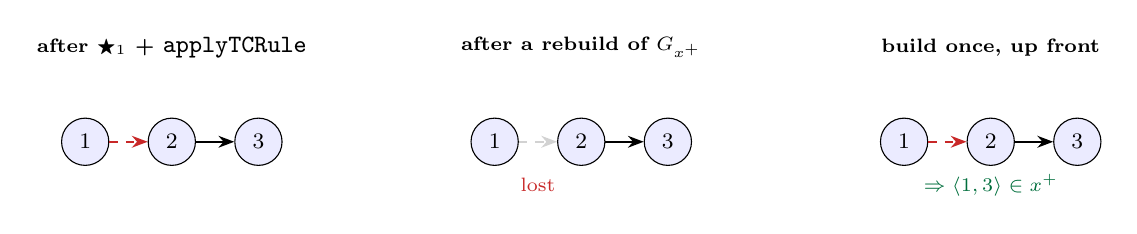
\begin{tikzpicture}[font=\footnotesize,
  n/.style={draw,circle,inner sep=1pt,minimum size=6mm,fill=blue!8},
  base/.style={-{Stealth[length=2mm]},thick},
  clos/.style={-{Stealth[length=2mm]},thick,dashed,hl},
  lbl/.style={font=\scriptsize\bfseries}]
  \begin{scope}
    \node[lbl] at (1.1,1.2) {after $\bigstar_1$ + \fn{applyTCRule}};
    \node[n] (a1) at (0,0) {$1$}; \node[n] (b1) at (1.1,0) {$2$};
    \node[n] (c1) at (2.2,0) {$3$};
    \draw[clos] (a1)--(b1); \draw[base] (b1)--(c1);
  \end{scope}
  \begin{scope}[xshift=5.2cm]
    \node[lbl] at (1.1,1.2) {after a rebuild of $G_{\tc{x}}$};
    \node[n] (a2) at (0,0) {$1$}; \node[n] (b2) at (1.1,0) {$2$};
    \node[n] (c2) at (2.2,0) {$3$};
    \draw[base] (b2)--(c2);
    \draw[clos,gray!35] (a2)--(b2);
    \node[hl,font=\scriptsize] at (0.55,-0.55) {lost};
  \end{scope}
  \begin{scope}[xshift=10.4cm]
    \node[lbl] at (1.1,1.2) {build once, up front};
    \node[n] (a3) at (0,0) {$1$}; \node[n] (b3) at (1.1,0) {$2$};
    \node[n] (c3) at (2.2,0) {$3$};
    \draw[clos] (a3)--(b3); \draw[base] (b3)--(c3);
    \node[good,font=\scriptsize] at (1.1,-0.55) {$\Rightarrow \tup{1,3}\in\tc{x}$};
  \end{scope}
\end{tikzpicture}
\caption{What Observation~\ref{obs:destroy} would cost on the benchmark of
Section~\ref{sec:repro}: rebuilding $G_{\tc{x}}$ after \fn{applyTCRule} has run
loses the edge $1\to2$, and with it the only path from 1 to 3.}
\end{figure}

\begin{observation}[Cost]
When $\bigstar_2$ does fire --- for every closure term the guards have not
already marked --- it is $O(|\mathit{members}(r)|)$ node constructions and map
insertions per closure term per full-effort round, including one
\code{RelsUtils::constructPair} \code{APPLY\_CONSTRUCTOR} node per member, which
goes through the node manager's hash-consing table. Phase~0 does that work
exactly once instead, and the guard lookups on the hot path of
\fn{applyTCRule} --- three map searches and a \fn{getRepresentative} per
(membership, closure term) pair --- disappear with it. It is not dominant, and
Section~\ref{sec:measure} finds it unmeasurable.
\end{observation}

\section{The benchmarks that exercise the interaction}\label{sec:repro}

\begin{lstlisting}[style=smt]
; EXPECT: unsat
(set-logic ALL)
(declare-fun x () (Relation Int Int))
; base edge: (2,3) in x, hence (2,3) in (rel.tclosure x)
(assert (set.member (tuple 2 3) x))
; closure edge not derivable from x alone
(assert (set.member (tuple 1 2) (rel.tclosure x)))
; transitivity of the two forces (1,3) in (rel.tclosure x)
(assert (not (set.member (tuple 1 3) (rel.tclosure x))))
(check-sat)
\end{lstlisting}

\noindent
This is exactly \textsc{TClos Up I} followed by \textsc{TClos Up II}, i.e.\
Example~3 of the paper with one of the two premises moved from $R$ to $\tc{R}$.
The problem is trivially unsatisfiable, and it is the smallest formula in which
$G_{\tc{x}}$ has to hold a base edge and a closure edge at the same time: lose
the closure edge $1\to2$ and \fn{doTCInference} can only re-derive
$\tup{2,3}\in\tc{x}$, leaving the solver to split the \textsc{TClos Down}
disjunction of \fn{applyTCRule} over freshly reachable Skolems for ever.
\file{regress1/rels/tc-overwrite-bug.smt2} is the same formula, added to the
suite by PR~\#12793.

Four variations pin the shape down. All were run on the same Debug build with a
20\,s limit; both configurations answer all five correctly, which is the point
--- \code{main}'s guards and Phase~0 protect the same edges.

\begin{center}\small
\renewcommand{\arraystretch}{1.15}
\begin{tabular}{@{}llcc@{}}
\toprule
& & \multicolumn{2}{c}{result / time}\\
\cmidrule(l){3-4}
Benchmark & Shape & \code{main} & once\\
\midrule
A \code{repro} & $\tup{2,3}\in x$, $\tup{1,2}\in\tc{x}$, $\tup{1,3}\notin\tc{x}$
  & unsat 0.013\,s & unsat 0.012\,s\\
B \code{no-base-member} & as A but $\tup{2,3}\in\tc{x}$ instead of $\in x$
  & unsat 0.011\,s & unsat 0.011\,s\\
C \code{all-base} & $\tup{1,2},\tup{2,3}\in x$, $\tup{1,3}\notin\tc{x}$
  & unsat 0.010\,s & unsat 0.009\,s\\
D \code{sat-no-path} & $\tup{3,4}\in x$, $\tup{1,2}\in\tc{x}$, $\tup{1,4}\notin\tc{x}$
  & sat 0.011\,s & sat 0.010\,s\\
E \code{chain4} & $1\!\to\!2\,(\tc{x})$, $2\!\to\!3\,(x)$, $3\!\to\!4\,(\tc{x})$,
  $4\!\to\!5\,(x)$, $\tup{1,5}\notin\tc{x}$
  & unsat 0.010\,s & unsat 0.010\,s\\
\bottomrule
\end{tabular}
\end{center}

\begin{itemize}[leftmargin=*,itemsep=1pt]
\item \textbf{B} isolates the \code{members.size() > 0} guard inside
  \fn{buildTCGraphForRel}. Moving the one base membership into the closure makes
  $r$ memberless, so a rebuild would store nothing and could not overwrite
  anything; the closure edges survive with or without protection.
\item \textbf{C} is Example~3 of~\cite{MRT17} verbatim: all edges are base
  edges, so no closure-only edge is ever at risk.
\item \textbf{D} checks that neither configuration \emph{over}-infers: there is
  no path from 1 to 4, the problem is satisfiable, and both say \textsf{sat}.
\item \textbf{E} is the same interaction over a four-edge path, i.e.\ with two
  closure edges to preserve rather than one.
\end{itemize}

\subsection{The in-tree regression that used to be disabled}
\label{sec:reltc7}

\file{test/regress/cli/\allowbreak{}regress0/rels/\allowbreak{}rel\_tc\_7.cvc.smt2}
is the same interaction reached through a join:

\begin{lstlisting}[style=smt]
; EXPECT: unsat
(set-logic ALL)
(declare-fun x () (Relation Int Int))
(declare-fun y () (Relation Int Int))
(assert (= y (rel.join (rel.tclosure x) x)))
(assert (set.member (tuple 1 2) (rel.join (rel.join x x) x)))
(assert (not (set.subset y (rel.tclosure x))))
(check-sat)
\end{lstlisting}

\noindent
until recently \file{test/regress/cli/CMakeLists.txt} listed it in
\code{regression\_disabled\_tests}:

\begin{lstlisting}[style=smt,language=]
  # timeout after fixing upwards closure for relations
  regress0/rels/rel_tc_7.cvc.smt2
\end{lstlisting}

\noindent
\code{git show 3bcc47a3c -- test/regress/CMakeLists.txt} shows that this very
line was added by PR~\#7515, whose description says as much: \emph{``It disables
a regression that times out after these fixes.''} The join and the outer closure
put memberships into both $x$'s class and $\tc{x}$'s class, which is benchmark~A
again, so protecting the closure edges is exactly what the test needs.

\begin{center}\small
\begin{tabular}{@{}lll@{}}
\toprule
Configuration & \code{rel\_tc\_7.cvc.smt2} & Time\\
\midrule
\code{main} (\code{5cc03f4b9}) & \textbf{unsat} & 0.01\,s\\
once (\code{8bcdf3239})        & \textbf{unsat} & 0.01\,s\\
\bottomrule
\end{tabular}
\end{center}

\noindent
It has been passing since PR~\#12793 landed, but nobody noticed, so it stayed
disabled. Commit \code{8bcdf3239} moves it out of
\code{regression\_disabled\_tests} into \code{regress\_0\_tests}, where it passes
in 0.13\,s under \fn{ctest} and also under \code{--check-proofs},
\code{--check-unsat-cores} and \code{--produce-proofs
--proof-granularity=theory-rewrite}, which is what the other CI configurations
run. Nothing else in the disabled list changes:
\code{regress1/rels/garbage\_collect.cvc.smt2} still times out in both
configurations.

\section{The patch}

\begin{enumerate}[leftmargin=*,itemsep=1pt]
\item Add an unconditional pass at the top of \fn{check()} --- i.e.\ immediately
  after \fn{collectRelsInfo} in the caller --- that builds the graph of every
  closure term once (Phase~0 of Algorithm~\ref{alg:check}).
\item Delete $\bigstar_1$ from \fn{applyTCRule} (and the now-pointless
  \code{d\_rel\_nodes.insert(tc\_rel)}).
\item Delete $\bigstar_2$ from Phase~B --- the whole branch, guard included, so
  that Phase~B no longer has a \textsc{tclosure} case at all.
\item While there: make \fn{buildTCGraphForRel} look the membership list up
  with \code{find} instead of \code{operator[]}, so that it stops inserting
  empty entries into the two maps Phase~A iterates, and drop the unused
  \code{tc\_rel\_rep}.
\end{enumerate}

\begin{lstlisting}
// --- in TheorySetsRels::check(), before Phase A -------------------------
// Build the transitive closure graph of every RELATION_TCLOSURE term before
// any rule is applied.
//
// buildTCGraphForRel reads only d_rReps_memberReps_cache,
// d_rReps_memberReps_exp_cache and the equality engine. The two caches are
// filled by collectRelsInfo above and are not written by any rule, and the
// rules only queue pending lemmas (see sendInfer), so representatives do not
// change either. The graphs built here are therefore exactly the graphs the
// rules below would have built lazily.
//
// Building them here, once per tc term, is what makes the graphs stable:
// applyTCRule adds the memberships of TC(r) itself to d_tcr_tcGraph, and any
// later call to buildTCGraphForRel would overwrite that graph with the base
// members of r alone, so those edges would never reach doTCInference and the
// TCLOSURE-UP II (transitivity) inferences would be lost.
for (const std::pair<const Node, std::map<Kind, std::vector<Node> > >& t :
     d_terms_cache)
{
  std::map<Kind, std::vector<Node> >::const_iterator tc_it =
      t.second.find(Kind::RELATION_TCLOSURE);
  if (tc_it != t.second.end())
  {
    for (const Node& tc_rel : tc_it->second) { buildTCGraphForRel(tc_rel); }
  }
}

// --- in buildTCGraphForRel ---------------------------------------------
MEM_IT mem_it = d_rReps_memberReps_cache.find(rel_rep);
if (mem_it == d_rReps_memberReps_cache.end())
{
  // tc_rel[0] has no asserted members, nothing to build
  return;
}
const std::vector<Node>& members = mem_it->second;
\end{lstlisting}

\noindent
The header documentation of \code{d\_rRep\_tcGraph} and \fn{buildTCGraphForRel}
is updated in the same commit: PR~\#12793 had documented \code{d\_rRep\_tcGraph}
as doubling as a ``graph already built'' marker that callers must test, which is
no longer true of either map.

\noindent
Ordering matters: the pass must run \emph{before} Phase~A, because
\fn{applyTCRule} consults \code{d\_rRep\_tcGraph} through \fn{isTCReachable} to
decide whether to skip the expensive splitting lemma, and it appends to
\code{d\_tcr\_tcGraph}.

\noindent
Deleting the Phase~B branch \emph{entirely} matters, rather than keeping it and
dropping its now-apparently-redundant guard. Phase~0 makes the \emph{build}
redundant; it never makes the overwrite harmless, because \fn{applyTCRule} has
run in between (Observation~\ref{obs:destroy}). A call site protected only by
bookkeeping state is an invitation to exactly that mistake, which is the
strongest argument for not having one.

\subsection{Why not keep the guards?}\label{sec:whynotguards}

\code{main}'s arrangement --- keep both lazy call sites, protect the graph with
the \code{d\_rel\_nodes} and \code{d\_rRep\_tcGraph} markers --- is the smaller
change, and it works. Three things make the up-front pass the better resting
place:

\begin{itemize}[leftmargin=*,itemsep=1pt]
\item It removes the $\bigstar_1$ guard's representative bug. That guard tests
  \code{d\_rReps\_memberReps\_cache.find(tc\_rel[0])} while
  \fn{buildTCGraphForRel} looks up $\rep{\code{tc\_rel[0]}}$, so when $r$ is not
  its own representative $\bigstar_1$ does not fire: \fn{isTCReachable} sees no
  graph during Phase~A and \fn{applyTCRule} emits a \textsc{TClos Down} splitting
  lemma for a membership the graph would have discharged. Phase~0 always has the
  graph in place before the first membership is processed.
\item It replaces two call sites and a four-clause condition, whose correctness
  depends on Phase~A preceding Phase~B, with ``built once, before any rule, then
  only added to'' --- Invariant~\ref{inv:complete}, for every closure term rather
  than one per base representative.
\item It saves the redundant build and the per-membership guard lookups
  (Observation~\ref{obs:destroy}). Phase~B visited every closure term anyway, so
  nothing new is computed.
\end{itemize}

\section{Measurement}\label{sec:measure}

\subsection{Setup}

What has to be shown is the opposite of a win: that replacing the guards with
Phase~0 changes \emph{nothing} observable. Both binaries were built in the same
tree, \code{5cc03f4b9} for \code{main} and \code{8bcdf3239} for once
(\code{CMAKE\_BUILD\_TYPE=Debug}, \code{ENABLE\_TRACING=ON}, Apple clang on
macOS/arm64). Absolute times are therefore much larger than a production build
would give; only the comparison between the two columns is meaningful.

\begin{sidenote}
A methodology trap worth recording, because it produced a completely wrong
first set of numbers. cvc5 builds \code{bin/cvc5} against
\code{@rpath/libcvc5.1.dylib} with an \code{LC\_RPATH} pointing at the
\emph{absolute} build directory. Copying only \code{build/bin/cvc5} aside and
then rebuilding makes the copied ``old'' executable load the \emph{new}
library, so both binaries run the same code and every benchmark looks
identical. Each configuration must be snapshotted together with
\code{libcvc5.1.dylib} and \code{libcvc5parser.1.dylib}, with
\code{install\_name\_tool} rewriting the rpath to the snapshot directory (and
an ad-hoc \code{codesign} afterwards on macOS).
\end{sidenote}

\subsection{Answers and inference counts}

The sharpest available check is not pass/fail but the per-inference counters:
two configurations that emit the same number of lemmas of every
\code{InferenceId}, on every benchmark, are doing the same reasoning. The
comparison covers all 100 in-tree \file{regress0/rels} and \file{regress1/rels}
benchmarks plus the 67 generated closure benchmarks of
\file{benchmarks/gen\_stress.py} (below), 20\,s limit each, comparing the answer
line and the whole
\code{theory::sets::inferences}\slash\code{inferencesLemma} histogram.

\begin{center}\small
\renewcommand{\arraystretch}{1.2}
\begin{tabular}{@{}lc@{}}
\toprule
& \code{main} vs once\\
\midrule
benchmarks compared                          & 167\\
\quad of which return a definitive answer    & 165\\
answers differing                            & \textbf{0}\\
\code{theory::sets} inference histograms differing & \textbf{0}\\
\midrule
\fn{ctest} \code{-R rels} (with \code{rel\_tc\_7} re-enabled) & 99/99 pass\\
\fn{ctest} \code{-R "sets|rels|relation"}                     & 303/303 pass\\
\bottomrule
\end{tabular}
\end{center}

\noindent
The two non-definitive benchmarks are the same in both configurations: the
expected parse error of \code{issue11903-join-unit-tuple.smt2} and the timeout
of the disabled \code{garbage\_collect.cvc.smt2}.

\subsection{Scaling families}

The in-tree closure benchmarks are all tiny, so seven families were generated at
$N \in \{4,8,16,32,64\}$ to put load on the code that Phase~0 touches:
\code{base-chain} (a chain of $N$ base edges, query at the far end),
\code{closure-chain} (the same chain asserted in $\tc{x}$ instead),
\code{mixed-chain} (alternating, i.e.\ the shape that needs the edges
\fn{applyTCRule} contributes), \code{clique} (edges $i\to i+1$ and $i\to i+2$),
\code{eqrel} (three provably equal base relations), \code{sat-chain} (a
satisfiable query) and \code{join-tc} (the \code{rel\_tc\_7} shape at size $N$).
Times are the wall clock of the largest instance of each family; the last row is
all 67 generated benchmarks, including the equal-relation probes of the next
subsection.

\begin{center}\small
\renewcommand{\arraystretch}{1.15}
\begin{tabular}{@{}lccc@{}}
\toprule
Family, $N=64$ & \code{main} & once & ratio\\
\midrule
\code{base-chain}    & 0.210\,s & 0.208\,s & 1.01\\
\code{closure-chain} & 0.231\,s & 0.234\,s & 0.99\\
\code{mixed-chain}   & 0.223\,s & 0.221\,s & 1.01\\
\code{clique}        & 0.564\,s & 0.559\,s & 1.01\\
\code{eqrel}         & 0.213\,s & 0.211\,s & 1.01\\
\code{sat-chain}     & 1.210\,s & 1.208\,s & 1.00\\
\code{join-tc}       & 2.283\,s & 2.241\,s & 1.02\\
\midrule
all 67 generated     & 8.663\,s & 8.594\,s & \textbf{1.01}\\
\bottomrule
\end{tabular}
\end{center}

\noindent
There is no measurable difference, and none should be expected: the work Phase~0
removes is a handful of map lookups per membership (the $\bigstar_1$ guard) and
one wasted rebuild per closure term whose base relation has members, against a
solve time dominated by the $O(N^2)$ \textsc{TClos Up} lemmas that
\fn{doTCInference} emits either way.

\subsection{The one case where once could do more work}

Phase~0 builds one graph per closure \emph{term}; \code{main}'s guards admit at
most one build per base \emph{representative}. Where several closure terms sit
over provably equal base relations, Phase~0 therefore populates
\code{d\_tcr\_tcGraph} for all of them and \fn{doTCInference} walks each --- $k$
times the forward inferences instead of one. Two probes bound the risk:

\begin{itemize}[leftmargin=*,itemsep=2pt]
\item Three families were generated with $k$ closure terms over base relations
  asserted equal: \code{eqwide} (plain top-level equalities, $k \in
  \{2,4,8,16\}$, $N \in \{16,32,64\}$), \code{eqterm} (each closure term pinned
  by an auxiliary relation $t_k = \tc{x_k}$, same grid) and \code{eqsat}
  (equalities entailed only at the SAT level, so the preprocessor cannot
  substitute them, $k \in \{1,2,4,8\}$, $N \in \{16,32\}$). The 24 instances of
  the first two total 2.311\,s and 2.300\,s, a ratio of 1.01 like everything
  else and flat in $k$; on \code{eqsat} the
  \code{SETS\_RELS\_TCLOSURE\_FWD} count is 528 at $N=32$ in both, and
  \emph{independent of $k$}, which is the tell. Tracing with
  \code{--trace=rels-debug} confirms it: preprocessing collapses the equal
  relations and \fn{check()} still reports ``\code{Check 1 terms of kind
  rel.tclosure}''.
\item Across all 100 in-tree \file{rels} benchmarks, no equivalence class ever
  contains more than one \code{rel.tclosure} term.
\end{itemize}

\noindent
So the case is real in principle and did not occur once in anything measurable.
Should it ever matter, the fix is to key Phase~0 by base representative, which
recovers \code{main}'s work profile without reintroducing a second call site.

\subsection{Differential fuzzing against an exact oracle}

The in-tree suite barely exercises the combination of a base edge and a closure
edge in the same graph, so a targeted random test was added. Formulas have the
shape
\begin{center}\small
$\{\tup{u_i,v_i}\in x\}_{i\in I}\;\cup\;\{\tup{u_j,v_j}\in\tc{x}\}_{j\in J}
 \;\cup\; \{\tup{a,b}\notin\tc{x}\}$
\end{center}
over pairwise-distinct integer constants, with $2$--$7$ nodes and $1$--$10$
edges, biased so that both labels usually occur.

\paragraph{The oracle is exact.} Let $E$ be the union of both edge sets. In any
model, each asserted $x$-edge is in $x$ and each asserted $\tc{x}$-edge
$\tup{u,v}$ forces some $x$-path $u\leadsto v$; hence $b$ reachable from $a$ in
$E$ (in $\ge 1$ steps) implies $\tup{a,b}\in\tc{x}$, so the formula is
unsatisfiable. Conversely, taking $x$ to be the asserted $x$-edges plus one
direct edge per asserted $\tc{x}$-edge gives $\tc{x} = $ the transitive closure
of $E$, which is a model whenever $b$ is \emph{not} reachable from $a$ in $E$.
So
\[
  \text{formula unsatisfiable} \iff b \text{ reachable from } a \text{ in } E
  \text{ in } \ge 1 \text{ steps},
\]
which a five-line depth-first search decides. \emph{Any} disagreement with it is
a bug in one of the two configurations, so this test does not merely compare
them against each other.

\paragraph{Result} 900 instances over seeds 1--3, 8\,s limit each.

\begin{center}\small
\renewcommand{\arraystretch}{1.2}
\begin{tabular}{@{}lcc@{}}
\toprule
& \code{main} & once\\
\midrule
matches the oracle & 900 & 900\\
timeout            & 0   & 0\\
\emph{wrong answer}& \textbf{0} & \textbf{0}\\
answers differing between the two & \multicolumn{2}{c}{\textbf{0}}\\
\bottomrule
\end{tabular}
\end{center}

\noindent
Both configurations decide every instance the oracle decides, and neither ever
produced a wrong answer --- in particular, having the closure edges present never
turned a satisfiable instance into \textsf{unsat}, which is the failure mode to
worry about when a rule gets more to work with.

\section{Conclusion of the investigation}

\textbf{Building once, immediately after \fn{collectRelsInfo}, is better}, but
not for the reason one might expect: it is not a speedup and not a bug fix.
Against \code{main} the measurements say plainly that nothing observable changes
--- same answers, same inference histograms, same run times to within noise
(Section~\ref{sec:measure}). The case is structural:

\begin{enumerate}[leftmargin=*,itemsep=2pt]
\item \textbf{The invariant becomes checkable by inspection.}
  Invariant~\ref{inv:complete} --- ``$G_T$ is built exactly once, before any rule
  runs, and is only ever added to afterwards'' --- holds by construction, for
  every closure term. \code{main} establishes something weaker (per base
  representative, and only because Phase~A happens to precede Phase~B), and it
  spends two call sites and a four-clause condition doing it.
\item \textbf{It removes the coupling of correctness to bookkeeping state.}
  \code{d\_rel\_nodes} and \code{d\_rRep\_tcGraph} stop doubling as
  ``already built'' markers. That coupling is the kind that fails quietly: the
  protection is invisible at the call site, so the next person to work on
  Phase~B can reasonably conclude the condition is a redundant optimisation and
  drop it, and no test they are likely to run will complain until a formula
  asserts memberships in both $r$ and $\tc{r}$.
\item \textbf{It removes a latent representative bug} in the $\bigstar_1$ guard
  (Section~\ref{sec:whynotguards}), and stops \fn{buildTCGraphForRel} from
  mutating the membership maps through \code{operator[]}.
\item \textbf{It revives an in-tree regression.}
  \code{rel\_tc\_7.cvc.smt2} has been passing since PR~\#12793 and is re-enabled
  here (Section~\ref{sec:reltc7}), which puts the interaction under CI in every
  configuration rather than in a benchmark directory.
\end{enumerate}

\noindent
The only argument for keeping a lazy build is to avoid constructing graphs for
closure terms that no rule ever consults. That argument does not apply here:
Phase~C (\fn{doTCInference}) iterates \emph{all} of \code{d\_tcr\_tcGraph}
unconditionally, so every graph is consulted in every round anyway --- and
Phase~B built all of them already.

\section{Other rough edges noticed along the way}

None of these are addressed by the patch; they are recorded because a newcomer
will trip over them.

\begin{enumerate}[leftmargin=*,itemsep=2pt]
\item \fn{doPendingInfers} is declared in the header and never defined;
  \fn{processInference} is defined and never called; the header comments refer
  to a \code{d\_pending} vector that does not exist.
\item The header declares \fn{applyJoinImageRule}\code{(Node mem\_rep, Node
  rel\_rep, Node exp)} and \fn{applyIdenRule}\code{(Node mem\_rep, Node
  rel\_rep, Node exp)}, but both are called with the \emph{operator term}, not
  a representative, and the definitions name the parameter accordingly.
\item \code{start\_node\_rep} in the recursive \fn{doTCInference} and the
  \code{*\_rel\_rep} parameters of \fn{applyTransposeRule},
  \fn{applyProductRule}, \fn{applyJoinRule} and \fn{applyTCRule} are unused
  except in trace output. (\code{tc\_rel\_rep} in \fn{buildTCGraphForRel} was
  the same and is gone as of \code{8bcdf3239}.)
\item \fn{doTCInference} dereferences
  \code{rel\_tc\_graph\_exps.find(new\_pair)->second} without checking for
  \code{end()} (Invariant~\ref{inv:tot}).
\item \fn{applyTransposeRule}\code{(vector)} is invoked once per member of the
  equivalence class although its conclusion does not depend on the member.
\item The DFS in \fn{isTCReachable} does not stop early once the target is
  found.
\end{enumerate}

%%==========================================================================
\appendix
\section{Quick reference: file map}

All line numbers in this document refer to \file{src/theory/sets/theory\_sets\_rels.cpp}
at commit \code{8bcdf3239} (branch \code{build-trc-graph-once}), except in
Part~\ref{part:tc} where a passage quotes \code{main} (\code{5cc03f4b9}).

\begin{center}\small
\renewcommand{\arraystretch}{1.1}
\begin{longtable}{@{}rlp{9.4cm}@{}}
\toprule
Line & Function & Role\\
\midrule\endhead
57  & \fn{check(Effort)}                    & entry point; full effort only\\
75  & \fn{check()}                          & Phase 0 / A / B / C driver, Alg.~\ref{alg:check}\\
252 & \fn{collectRelsInfo}                  & rebuild indices from the equality engine\\
343 & \fn{computeMembersForJoinImageTerm}   & join image, up\\
468 & \fn{applyJoinImageRule}               & join image, down\\
542 & \fn{applyIdenRule}                    & identity, down\\
584 & \fn{computeMembersForIdenTerm}        & identity, up\\
648 & \fn{applyTCRule}                      & \textsc{TClos Down} + graph augmentation\\
761 & \fn{isTCReachable}                    & entailment guard (2 overloads)\\
830 & \fn{buildTCGraphForRel}               & materialise $G_{\rep r}$ and $G_T$\\
879 & \fn{doTCInference}$(G,E,T)$           & per-graph path enumeration\\
918 & \fn{doTCInference}(recursive)         & DFS, builds the explanation chain\\
1008& \fn{applyProductRule}                 & \textsc{Prod Down}\\
1072& \fn{applyJoinRule}                    & \textsc{Join Down} + redundancy check\\
1153& \fn{applyTableJoinRule}               & table join, down\\
1222& \fn{applyTransposeRule}(vector)       & \textsc{Transp Eq}\\
1243& \fn{applyTransposeRule}(rel,rep,exp)  & \textsc{Transp Down}\\
1274& \fn{doTCInference}()                  & Phase C driver\\
1295& \fn{computeMembersForBinOpRel}        & recurse into args, then compose\\
1355& \fn{computeMembersForUnaryOpRel}      & \textsc{Transp Up}\\
1413& \fn{composeMembersForRels}            & \textsc{Join Up} / \textsc{Prod Up}\\
1526& \fn{applyTableJoinUp}                 & table join, up\\
1613& \fn{processInference}                 & (dead) entailment-checked assert\\
1643& \fn{areEqual}                         & recursive on tuples; marks shared terms\\
1683& \fn{safelyAddToMap}                   & semantic de-duplication of members\\
1712& \fn{makeSharedTerm}                   & request a proxy singleton\\
1730& \fn{computeTupleReps}                 & memoise a tuple's representative vector\\
1746& \fn{reduceTupleVar}                   & replace a tuple variable by a constructor\\
1774& \code{TupleTrie::*}                   & the membership index\\
1901& \fn{sendInfer}                        & enqueue $\mathit{reason}\Rightarrow \mathit{fact}$\\
\bottomrule
\end{longtable}
\end{center}

\section{Reproducing the experiment}

\begin{lstlisting}[style=smt,language=]
# Snapshot a configuration together with its shared libraries, otherwise the
# copied executable will load whatever libcvc5.dylib is in build/src later on.
# Keeping the build tree's own bin/ src/ src/parser/ layout means a single
# -rpath rewrite per entry is enough.
snapshot() {                      # $1 = destination directory
  R=$PWD; d=$1; rm -rf $d; mkdir -p $d/bin $d/src/parser
  cp    $R/build/bin/cvc5                       $d/bin/
  cp -R $R/build/src/libcvc5*.dylib             $d/src/
  cp -R $R/build/src/parser/libcvc5parser*.dylib $d/src/parser/
  install_name_tool -rpath $R/build/src        $d/src \
                    -rpath $R/build/src/parser $d/src/parser $d/bin/cvc5
  codesign -f -s - $d/bin/cvc5                  # required on arm64
}

git stash                                       # baseline = main
ninja -C build cvc5-bin && snapshot /tmp/base
git stash pop                                   # once
ninja -C build cvc5-bin && snapshot /tmp/once

# Both configurations answer everything, so compare the answers *and* the
# per-InferenceId histograms, which is the sensitive check.
python3 rels-guide/benchmarks/gen_stress.py /tmp/stress    # 67 benchmarks
for f in test/regress/cli/regress[01]/rels/*.smt2 /tmp/stress/*.smt2; do
  a=$(/tmp/base/cvc5 --tlimit=20000 --stats $f 2>&1 \
        | grep -E '^(sat|unsat|unknown)|theory::sets::inferences' | sort)
  b=$(/tmp/once/cvc5 --tlimit=20000 --stats $f 2>&1 \
        | grep -E '^(sat|unsat|unknown)|theory::sets::inferences' | sort)
  [ "$a" = "$b" ] || echo "DIFF $f"
done

BASE_BIN=/tmp/base/bin/cvc5 ONCE_BIN=/tmp/once/bin/cvc5 \
  MAX_NODES=7 MAX_EDGES=10 \
  python3 rels-guide/benchmarks/fuzz_tc.py 1 300     # seeds 1, 2, 3
\end{lstlisting}

\begin{thebibliography}{9}
\bibitem{MRT17}
B.~Meng, A.~Reynolds, C.~Tinelli, C.~Barrett.
\newblock \emph{Relational Constraint Solving in SMT}.
\newblock CADE-26, LNCS 10395, Springer, 2017.
\newblock (\file{MRT+17.pdf}; the calculus of Section~\ref{sec:calculus} is
Figures 2 and 3 of that paper.)

\bibitem{Bansal16}
K.~Bansal, A.~Reynolds, C.~W.~Barrett, C.~Tinelli.
\newblock \emph{A New Decision Procedure for Finite Sets and Cardinality
Constraints in SMT}.
\newblock IJCAR 2016, LNCS 9706, pp.~82--98.

\bibitem{PR7515}
A.~Reynolds. \emph{Fix upwards closure for relations}, cvc5 PR \#7515,
commit \code{3bcc47a3c}, November 2021.
\end{thebibliography}

\end{document}
